\documentclass[11pt,a4paper]{amsart}
\usepackage{geometry, empheq}
\usepackage[english]{babel}
%\pagestyle{myheadings}
%\textheight25.3cm
%\oddsidemargin 1cm
%\evensidemargin 1cm
\usepackage{amsmath, mathabx}
%\usepackage{showkeys}
\usepackage{amssymb}
\usepackage{amsthm}
\usepackage{xcolor,graphicx}
\usepackage{color}
\usepackage{varioref}
\usepackage{nicefrac}
\usepackage{caption}
\usepackage{subcaption}
\usepackage{float}
\usepackage[normalem]{ulem}
\usepackage{multirow}
\usepackage{enumerate}
\usepackage[colorinlistoftodos]{todonotes}
\usepackage{amsfonts}
\usepackage{booktabs}
\usepackage{siunitx}
%\usepackage{hyperref}
\usepackage{pgfplots} 
\usepackage{pgfplotstable}
\usepackage{tikz}
%\usepackage{pdflscape}
%\usepackage{pgfgantt}
%\usepackage{pdflscape}
%\usepgfplotslibrary{external} 
%\tikzexternalize
%\pgfplotsset{compat=newest} 
%\pgfplotsset{plot coordinates/math parser=false}
\usepackage{algorithm}
\usepackage{algorithmic}
\usepackage{comment}
\usepackage{caption}
\captionsetup{skip=5pt}
%\usepackage{url}

%\selectcolormodel{gray}
\def\b#1{{\mbox{\boldmath $#1$}}}
\def\lewz#1{\leqno(#1)}
%\usepackage{booktabs}
\newcommand{\ak}{\hspace{20pt}}
\newcommand{\bak}{\parindent=0pt}
\newcommand{\sm}{\smallskip}
%\newcommand{\smallskip}{\medskip}
\newcommand{\bs}{\bigskip}
\newcommand{\arrow}{\rightarrow}
\newcommand{\ds}{\displaystyle}
\newcommand{\kr}{\hspace{-0.2cm}{\bf.~}}
\newcommand{\kw}{\rule{2mm}{2mm}}
\newcommand{\ged}{\hfill\kw}
\newcommand{\pf}{\b{Proof.} \ }
\newcommand{\ssn}{({\bf SSN}) }
\renewcommand{\div}{\text{div\,}}
\newtheorem{example}{\textbf{Example}}
%\newcommand{\norm}[1]{{\|  #1\|}}
\renewcommand{\l}{\left}
\renewcommand{\r}{\right}
\newcommand{\om}{\Omega}
\newcommand{\ga}{\Gamma}
\newcommand{\fsparse}{\Upsilon}
\newcommand{\reals}{\mathbb{R}}
\newcommand{\sign}{\mathrm{sign}}
\newcommand{\warrow}{\rightharpoonup}
\def\thesection{\arabic{section}}
\def\thesubsection{\arabic{section}.\arabic{subsection}}
\def\thefigure{\arabic{figure}\normalfont}
\def\thetable{\arabic{table}\normalfont}
\setcounter{table}{0}
\newcommand{\nota}[1]{ \colorbox{red}{\textcolor{white}{\tiny{#1}}}}
\DeclareMathOperator{\argmin}{argmin}
%\newenvironment{proof}[1][Proof]{\b{Proof.}{\hfill\kw}}
\renewenvironment{proof}{{Proof.}}{\hfill\kw}

%\font\nowa = eufm5 scaled \magstep 3
\font\tenpoint=cmr10
\font\ninepoint=cmr9
\newcounter{theassumption}
\setcounter{theassumption}{0}
\newtheorem{assumption}[theassumption]{{Assumption}}
\newtheorem{proposition}{{Proposition}}
\newtheorem{definition}{{Definition}}
\newtheorem{lemma}{{Lemma}}
\newtheorem{remark}{{Remark}}
\newtheorem{corollary}{{Corollary}}
\newtheorem{theorem}{{Theorem}}
\newcommand{\cor}{\color{red}}
\newcommand{\norm}[1]{\lVert #1 \rVert}
\newcommand{\subtag}[1]{\tag{\theparentequation#1}}
%\addbibresource{biblio.bib}

\begin{document}
	\title[Nonconvex optimal control problems]{ Sparse elliptic optimal control problems with mixed control-state constraints}
	%\title{Numerical solution of nonconvex PDE--constrained optimization problems via DC programing}
	
	\author{Pedro Merino$^\ddag$ and Diego Vargas$^\ddag$}
	%\address{}
	\address{$^\ddag$Research Center of Mathematical Modeling (MODEMAT) and Department of Mathematics, Escuela Polit\'ecnica Nacional, Quito, Ecuador}
	\keywords{}
	\subjclass[2010]{90C26, 90C46, 49J20, 49K20}
	\thanks{$^*$This research has been supported by Research Project PIMI-17-01 funded by Escuela Polit\'ecnica Nacional, Quito--Ecuador.}
	
	\smallskip
\begin{abstract}
In this paper we study a nonconvex optimal control problem with sparsity induced by a $L^q$-quasi norm penalty ($0<q<1$), and when mixed point wise constraints are imposed. We discuss the numerical solution of such problems, considering a method that combines the DC-Method (Difference-of-convex functions algorithm) together with the semi smooth Newton method, and which was derived from the optimality conditions of a regularized problem using the DC--programming approach.
\end{abstract}
	
\maketitle 

\tableofcontents



\section{Introduction}

In the theory of optimal control problems governed by partial differential equations, the utilization of penalties in the cost function which induces sparsity on the optimal control, and the presence of mixed--constrained restrictions over the control and state of the problem, are widely studied and used for many theoretical and practical problems, but in a separated way. However, as far as we know, there are few literature about problems which combines these two paradigms in only one optimal control problem, despite the relevance that each individual paradigm could represent. For example, problems with penalties using $L^q$ quasi norms, with $q\in [0,1)$ are well known for inducing sparcity over the optimal control solution, see for example \cite{ito-kunish, merino}, likewise the $L^1$ penalization in the cost function studied, for example, by Stadler \cite{stadler}; therefore, such characteristic over the optimal control could be used for placement of technological equipment, inverse problems in biomedical or seismic imaging, certain energy efficiency models (see \cite{vogel}), image restoration (see \cite{hinttv}), compressed sensing (see \cite{donoho}) and optimal control problems (see \cite{casas}). However, the main difficult in the treatment of the quasi-norm penalized problems is the obvious lack of convexity in the cost function, which implies that the use of standard techniques of the Convex Analysis cannot be applied for the derivation of a solution and an optimally system for it.\\ 

On the other hand, optimal control problems which present restrictions over the control and state are studied by several authors, see for example \cite{casas, casas-kunisch, casas-delosreyes}, etc. Those problems are important in practical uses, for example, problems involved with heat phenomena, elasticity theory, flux theory, finances and over all problems which demands that the state must be in specific set \cite{hintkun}. However, when we impose point-wise state constrains in some optimal control problems with convex cost function, it was shown that the Lagrange multipliers that appears in the optimal systems have poor regularity, see for example \cite{casas, casas-delosreyes}. This result introduces a new challenge in the study of this kind of problems, because the lack of sufficient regularity for the Lagrange multipliers arisen from the optimal system above implies that their numerical treatment could be difficult. Even the active-set strategies proposed by Bergounioux, Ito and Kunisch \cite{bik}, Bergounioux and Kunisch \cite{bk}, or Kunisch and Rosch \cite{kr}, cannot be applied for its numerical treatment. However, in \cite{meyer1} it is introduced a technique for witch we get a sub problem with $L^2$ Lagrange multipliers. This technique consists in defining an artificial control which involves the originals states and control of the problem and reformulate the original optimal control problem with the new artificial control. This process is called a \textit{Lavrentiev regularization} for the problem, and the main idea of this is to interchange the point-wise constrains from the original state to the new defined control.\\

 For the numerical analysis of problems with non convex penalties, it is frequently used a well-known technique called Newton's semi-smooth method, which was first introduced by Mifflin in \cite{mifflin} for the study of problems defined on finite-dimensional spaces, and then it was extended to problems on infinite dimensional spaces by Qi and Sun \cite{qi}, \cite{qisun}. The importance of the semi-smooth method lies in the fact that it can be applied to solve equations of the form $F(x)=0$, being $F$ some function or functional on a Banach space, imitating Newton's classical algorithm for solving equations; but the main difference between these two methods is that $F$ does not have necessary sufficient regularity, such as a $C^1$ regularity on its domain. For this reason, we use the theory of Newton semi smooth methods developed in \cite{ulbrich} in order to determinate the numerical solution of our problem particularized to a certain PDE equations. \\

In this work we study a certain type of optimal control problem which presents a $L^q$ quasi norm penalization, $q\in ]0,1[$, and mixed control and state point-wise constraints; being these restrictions inspired in a Lavrentiev-type mix of control and state point-wise restrictions. Specifically, we demonstrate that our problem has a solution which can be used for the study of another control problem with a $L^q$ penalization and pure state point-wise state constraints. Then, we derive an optimal system for the penalized problem with pure state point-wise constraints, using the theory of Difference of Convex functions. Finally we develop a numerical algorithm for solving it, using the semi smooth Newton scheme and then we present our numerical results.\\

This paper is organized as follows: in the Section 2 we introduce our problem and some useful notations for this work. In Section 3 we introduce a regularization of the $L^q$ penalty present in our control problem, using the so called Convex regularization or $\Gamma-$regularization (see \cite{eck}), for deducing optimal systems that will be used after. In section 4 we present a $L^q$ penalized control problem with only point-wise state constrains, which can be seen as a particular case of the problem present in Section 2. In this chapter also we study the existence of solutions for it, using the results developed in Section 3. In Section 5 we deduce optimally conditions for the $L^q$ penalized problem with only point-wise state constrains, using the DC theory (Difference of Convex functions theory, see \cite{merino, dihn}). In Section 6 we use the semi smooth Newton method for the numerical analysis of our results, using the optimal system deduced in Section 5. We finalize this paper with our conclusions.

 \section{Preliminaries}
Let $\om \in \reals^{n}$ be a bounded domain with $n=2, 3$ and with a Lipschitz boundary $\Gamma$ whose unit outward normal vector $\nu$ is defined in almost all $x \in \Gamma$. Let  $a_{ij}$ be Lipschitz continuous functions for all $i,j\in \{1,\cdots,n\}$  such that there exist a positive constant $\alpha>0$, such that
\begin{equation}\label{pdecondition}
    \sum_{i,j=1}^{n}a_{ij}(x)\xi_{i}\xi_{j} \ge \alpha\norm{\xi}^2, \quad \forall  (x,\xi)\in \om\times\reals^n
\end{equation}
Let $A$ be a second-order differential operator defined for any $y\in H^1(\om)$ as
\[
    Ay=-\sum_{i,j=1}^{n}\dfrac{\partial}{\partial x_j}\l(a_{ij} \dfrac{\partial}{\partial x_i}y\r)+a_0y,
\]
with $a_0\in L^{\infty}(\om)$, $a_0(x)\ge 0$ a.e. $x\in \om$, and let $a: H^1(\om)\times H^1(\om)\to \reals$ the standar bilinear and coercive form constructed from the definiton of $A$. It is a well known fact (see for example \cite{trol}) that, for every $u\in L^2(\om)$ there exists a unique $y\in H^{1}(\om)$ such that
\begin{equation}\label{weak_formulation}
    a(y,v)=(u,v)_{L^2(\om)},\quad \mbox{ for all }v\in H^1(\om),
\end{equation}
and, moreover, there exists a positive constant $c_{a}$ which depends only of $\om$ and such that
\begin{equation}\label{continuity_bilinear}
    \norm{y}_{H^1(\om)}\le c_{a}\norm{u}_{L^2(\om)}.
\end{equation}
Relations \eqref{weak_formulation} and \eqref{continuity_bilinear} allow us to introduce the solution operator $S:L^2(\om)\to H^1(\om)$ which, for every $u\in L^2(\om)$ we have that $y=Su$ is the solution for \eqref{weak_formulation} which satisfies also $\eqref{continuity_bilinear}$.\\

In addition, if we denote $a^*$ as the adjoint operator of $a$, then, we recall that \cite{trol} for every $w\in L^2(\om)$ there exists a unique $z\in H^1(\om)$ such that
\begin{equation}\label{weak_adjoint_formulation}
a^*(z,v)=(w,v)_{L^2(\om)},\quad \mbox{ for all }v\in H^{1}(\om),
\end{equation}
and there exists a positive constant $c^*_{a}$ which only depends on $\om$ and such that
\begin{equation}\label{continuity_adjoint_bilinear}
\norm{z}_{H^1(\om)}\le c^*_a\norm{w}_{L^2(\om)}.
\end{equation}
In a similar fashion we introduce the solution operator $S^*: L^2(\om)\to H^1(\om)$ such that, for every $w\in L^2(\om)$ we get $z=S^*(w)$ which satisfies \eqref{weak_adjoint_formulation} and \eqref{continuity_adjoint_bilinear}.

{\color{red} Introducir la formulación débil de la ecuación de estado, justificar la existencia de una solución única y la estimaciones de continuidad por Lax-Milgram}



\subsection{Notations}
We introduce some useful notations: first of all, the classic Lebesgue spaces of functions which are square integrable over $\om$ almost everywhere will be denoted with the usual notation $L^2(\Omega)$. The Sobolev space of functions in $L^2(\om)$ which have first weak derivatives which belongs to $L^2(\om)$ is denoted as usually: $H^1(\om)$.{\color{red} realmente usamos este último espacio?}.\\

{\color{red} introducir  el subdiferencial con la definición} We recall the definition of the subdifferential of a convex function (see for example \cite{combettes, rock, valkonen}). Let $X$ a Banach space and $f:X\to ]-\infty,\infty]$ a convex function. Let $x\in X$ such that $f(x)<+\infty$. Then, the subdifferential of $f$ at $x$ consist of the set:
\[
\partial f(x):=\{y\in X^*: f(z)-f(x)\ge \langle y,z-x\rangle_{X^*,X},\; \mbox{for all }z\in X\}.
\]
Let $U$ a subset of $X$, the \emph{indicator function} over $U$ is defined as
\[
\mathbf{I}_{U}(u)=\begin{cases}
    0,& u\in U,\\
    +\infty,&u\notin U,
\end{cases}
\]
for all $u\in U$. 

Let $f:X\to \mathbb{R}$, the \emph{convex conjugate} (also called the Fenchel conjugate, see for example \cite{rock}) of $f$ will be denote by $f^*$ and the biconjugate of $f$ will be denote by $f^{**}$. The \emph{convex envelope} of $f$ is defined (see \cite{combettes}) as
\[
\widecheck{f}:=\sup\{g:X\to \reals: g\mbox{ is convex and }g(x)\le f(x) \mbox{ for all }x\in X\}.
\]
For a function $f:X\to \mathbb{R}$, we define the positive and negative parts of $f$ as
\[
[f(x)]_{+}:=\max\{0,f(x)\},\qquad [f(x)]_{-}:=-\min\{0,f(x)\}.
\]
{\color{red} citar el resultado en que $f^**$ es la convexificación de $f$}
{\color{red} no creo que necesitemos espacios de banach, sino solamente $L^2$}
If $f:E\to F$, with $F$ a Banach space, is Fréchet differentiable at some $x\in E$, we will denote its derivative as $\nabla f(x)$. 

Finally, the projection operator $\mathcal{P}$ over a Hilbert space $H$ is defined as a function from $H$ to a subspace $V\subset H$ such that $\mathcal{P}(x):=\argmin_{y\in V}\norm{x-y}^2$.

\subsection{Formulation of the optimal control problem}
For given real positive constants  $\alpha$, $\beta$, $\lambda$ and $q\in (0,1)$ and $\lambda>0$, we are interested in the mixed control-state constrained optimal control problem:
\begin{equation}\label{plambda}\tag{$P_{\lambda}$}
    \begin{cases}
    \displaystyle\min_{(y,u)\in H^1(\om)\times L^2(\om)}\; J(y,u) := \frac{1}{2}\norm{y-y_d}^2_{L^2(\om)}+\frac{\alpha}{2}\norm{u}^2_{L^2(\om)}+\beta \int_{\om} |u|^{q}\; dx\\
    \mbox{subject to:}\\
    Ay(x)=u(x), \phantom{aaaaa} \mbox{in } \om,\\
    \partial_{\nu}y(x)=0, \phantom{aaaaaaaaaaaaa} \mbox{over } \Gamma,\\    
    y_a\le y(x)+\lambda u(x)\le y_b,\phantom{a} \mbox{almost all }x\in \Omega
    \end{cases}
\end{equation}
with $y_a, y_b$ real constants. 

\begin{remark}
    Mixed constraints are also motivated by the Lavrentiev type regularization in the presence of point-wise state constrains, see \cite{meyer1}. 
    The main reason behind this consideration can be explained as follows: first of all, if we define the problem $(P_0)$ as same as the problem $(P_{\lambda})$, except for the point-wise constraints that we replace by $$y_a\le y(x)\le y_b,\quad \text{for all } x\in \Omega.$$
    
     Thus, $P_{0}$ is a non convex problem with point-wise state constraints. Such problems are practically and theoretically interesting due to the optimal control sparsity properties and the applicability of the state constraints. However, since the cost function is not convex, the existence of a solution for $P_0$ cannot be followed by the usual direct methods. They require special techniques of regularization for the non convex term present in this cost function. 
\end{remark}
 
Nevertheless, the relation between the solutions of the regularized problem $P_0$ and the non regularized $P_0$ are not enough clear. We avoid this difficult following a different way for demonstrating solutions for the non regularized $P_0$. In the first place, we consider the family of regularized problems $P_{\lambda}$ with $\lambda>0$, using the so called  \textit{Convex regularization} or $\Gamma-$\textit{regularization} of the problem (see \cite{eck}). This method consists in the substitution of the original non convex cost function of \eqref{P} for a convex version of it, constructed from the convex envelope of the one dimensional non convex penalty presented in \eqref{P}. The virtue of using such problems is that the optimal systems arisen from each one, produces a sequence of multipliers with converges as $\lambda\to 0$ to certain functions which will be used for demonstrating that the non regularized problem $P_0$ has at least one solution.


\section{Convex relaxation of the optimal control problem}

Regarding the existence of solutions for $(P_\lambda)$, we emphasize that the presence of the nonconvex $L^q$-quasinorm prevents the use of direct method arguments. In the absence of state constraints, optimal control problems involving the $L^q$-quasinorm penalty can be treated as in \cite{ref1}, by deriving an optimality system described by a monotone operator that depends on the optimal variables. The maximal monotone extension of this operator allows to prove the existence of a generalized solution. This approach was initially applied in \cite{ref2} and later extended to incorporate $L^q$-quasinorm penalties. Furthermore, as pointed out in \cite{ref1}, this procedure is equivalent to a convex relaxation of the cost functional of the optimal control problem.

The consideration of state constraints complicate the description of the associated optimality system by means of a monotone operator. Therefore, we rely on a convex relaxation $(P^C_\lambda)$ of the problem $(P_\lambda)$, for which we can establish the existence of solutions. Under similar hypotheses regarding the structure of the adjoint state as in \cite{ref3}, we demonstrate that a particular solution of the relaxed optimal control problem indeed solves $(P^C_\lambda)$. This relaxation is also known as $\Gamma-$regularization, and essentially it consists in replacing the integrand term $\frac{\alpha}{2}|t|^2+\beta |t|^q$ in the cost function of $\eqref{P}$ by the Fenchel bi-conjugate of the one-dimensional function $h(t):=\frac{1}{2}|t|^2+\beta|t|^q$.

%Before the details of the procedure discussed above, we point out the following: by the elliptic condition \eqref{pdecondition} and the structure of the partial differential equation that governs \eqref{P} as same as the structure of the domain $\Omega$, we know (see \cite{trol}) for each $u\in L^2(\Omega)$ there exists a unique $y\in H^1(\Omega)$ such that the P.D.E. is full-filled. Therefore we can use the solution operator $y=Su$ defined for each $u\in L^2(\Omega)$. Moreover, if we consider that $u\in L^{\infty}(\Omega)\cap L^2(\Omega)$, we can use the compact embedding operator $E$ from $H^1(\Omega)$ to $L^2(\Omega)$ and defining $R=ES$ for which if $u$ is the control function to our problem, $y=Ru$ is the state associated to it. On the other hand, if we define the control $v=(\lambda I+R)u$, for $\lambda>0$ small enough, and since  $R$ is a compact operator, $\lambda I+R$ represents a Fredholm operator that has only countable many eigenvalues accumulating at $0$. Therefore, since $R$ is positive definite, we can define the invertible operator $B_{\lambda}:L^{2}(\om)\to L^{2}(\om)$ such that
%\[    B_{\lambda}v=B_{\lambda}(y+\lambda u)=(\lambda I+R)^{-1}(R+\lambda I)(u)=u;
%\]
%and by definition, obviously, $y=SB_{\lambda}v$. 


 
\begin{lemma}
    Let $f:\reals \to [0,\infty[$ an even function. Suppose that $f$ is convex and non-decreasing on $[0,\infty[$. Then, $f$ is convex in all $\reals$.
\end{lemma}
\begin{proof}
    We prove first that $f$ is convex on $]-\infty,0]$. In fact, let $x,y\le 0$. Since $f$ is even, for any $\lambda\in [0,1]$, \begin{align*}
        f(\lambda x+(1-\lambda)y)&=f(\lambda(-x)+(1-\lambda)(-y))\\
        &\le \lambda f(-x)+(1-\lambda)f(-y)\\
        &=\lambda f(x)+(1-\lambda)f(y).
    \end{align*}
    Now, take $x<0<y$. First of all, suppose that for $\lambda\in [0,1]$, $p_{\lambda}:=\lambda x+(1-\lambda)y\ge 0$, and call $p'_{\lambda}:=\lambda(-x)+(1-\lambda)y$. Then $0\le p_{\lambda}<p_{\lambda}'$, so, by the non decreasing property of $f$ in $[0,\infty[$, we get that $f(p_{\lambda})\le f(p'_\lambda)$. But, since $p_{\lambda}'$ is a convex combination of $-x$ and $y$, which they are both greater or equal than zero, we get that $f(p_{\lambda})\le \lambda f(-x)+(1-\lambda)f(y)=\lambda f(x)+(1-\lambda)f(y)$. Otherwise $-p_{\lambda}\ge 0$; but $-p_{\lambda}=\lambda(-x)+(1-\lambda)(-y)$. However, since $-y<y$, calling $p''_{\lambda}=\lambda(-x)+(1-\lambda)y$, we get that $0\le p_\lambda<p''_{\lambda}$. Therefore, $f(p_{\lambda})=f(-p_{\lambda})\le f(p''_{\lambda})\le \lambda f(-x)+(1-\lambda)f(y)=\lambda f(x)+(1-\lambda)f(y)$. This prove that $f$ is convex over $\reals$.\\

    
    
\end{proof}

{\color{red} En esta parte se debe introducir $h$ y su biconjugada $h^**$ justificando su cálculo 
\begin{lemma}\label{l:biconjugate}
    Let us consider the penalty integrand of the cost functional of $(P_\lambda)$, given by the function $h(t)=\frac{\alpha}{2}|t|^2+\beta |t|^q$ defined  for all $t\in \mathbb{R}$, and let $q\in ]0,1[$. Then, the function $\widehat{h}:\mathbb{R}\to \mathbb{R}$ defined by
    %
    \begin{equation}\label{biconjugate}
       \widehat{h}(t)=\begin{cases}
            h(t),&|t|\ge t^*,\\
            r^*|t|,&|t|<t^*,
        \end{cases}
    \end{equation}
where
\[
    t^*=\left(\frac{2\beta}{\alpha}(1-q)\right)^{\frac{1}{2-q}},
\]
and $r^*=\alpha t^*+\beta q(t^*)^{q-1}$, corresponds to the biconjugate of $h$. In addition, its convex subdifferential corresponds to
   \begin{equation}\label{sub_biconjugate}
       \partial \widehat{h}(t)=\begin{cases}
           \alpha t+\beta q |t|^{q-1}\sign(t), &|t|\ge t^*,\\                     
           r^*\sign(t), &|t|<t^*, t\ne 0,\\
           \eta\in [-r^*,r^*], &t=0.
       \end{cases}
   \end{equation}
\end{lemma}
}
\begin{proof}
    Accordingly to Proposition 13.14 (iv) in \cite{combettes}, we have that the convex envelope of $h$ satisfies the relation $(\widecheck{h})^*=h^*$, so $(\widecheck{h})^{**}=h^{**}$. Moreover, by Proposition 9.8 (i), we have that $\widecheck{h}$ is a convex and lower semicontinuous function, so, by the Fenchel Moreau Theorem (Theorem 13.32 in \cite{combettes}) we have $(\widecheck{h})^{**}=\widecheck{h}$. Therefore, instead of computing the biconjugate of $h^{**}$ through the definition of the biconjugation, it is sufficient to compute the convex envelope $\widecheck{h}$ of $h$, since $\widecheck{h}=(\widecheck{h})^{**}=h^{**}$.\\ 

    Now, We claim that $\widehat{h}$ is the convex envelope of $h$. In fact, $\widehat{h}$ is a continuous function since $t^*$ satisfies the equation $h(t^*)=t^*h'(t^*)$, so $\lim_{|t|\nearrow t^*}\widehat{h}(t)=r^*t^*=t^*h'(t^*)=h(t^*)=\widehat{h}(t^*)$. 

    The convexity of $\widehat{h}$ follows from Lemma 1. In fact, $\widehat{h}$ is clearly an even function. Moreover, it is non decreasing on $[0,\infty[$, because it is non decreasing in $[0,t^*]$ and $[t^*,\infty[$. In addition, notice that for all $t\in \reals$, 
    \begin{equation}\label{lemma1:ineq1}
         r^*|t|\le h(t). 
    \end{equation}
    
    In fact, if we consider the function $\varphi(t):=\frac{\alpha}{2}|t|+\beta|t|^{q-1}$ defined for all $t\in \mathbb{R}\setminus\{0\}$, we have that $|x|=t^*$ are the minimums for $\varphi$. Therefore, $\varphi(t^*)\le \varphi(t)$ for all $t\in \mathbb{R}\setminus\{0\}$. But, since $t^*$ satisfies the equation
    \[
    \alpha t^*+\beta q (t^*)^{q-1}=\frac{\alpha}{2}t^*+\beta(t^*)^{q-1},
    \]
    we have that $r^*=\varphi(t^*)\le \varphi(t)=\frac{\alpha}{2}|t|+\beta|t|^{q-1}$. Multiplying both sides of the last equation by $|t|$ follows the result. This last fact allow us to say that $\widehat{h}$ is non-decreasing in $[0,\infty[$. Moreover, since $\widehat{h}$ is a $C^1(\reals\setminus\{0\})$ function, and $\widehat{h}'$ is non decreasing in $]0,\infty]$, Proposition 8.12 in \cite{combettes} plus the continuity of $\widehat{h}$ at $0$, assures that $\widehat{h}$ is convex on $[0,\infty]$. Now, Lemma 1. establish the convexity of $\widehat{h}$ in $\reals$.\\   

    Finally, we claim that $\widehat{h}=\widecheck{h}$. In fact, we have seen that $\widehat{h}$ is convex, continuous, and $\widehat{h}(x)\le h(x)$ for all $x\in\mathbb{R}$, so by definition $\widehat{h}(x)\le \widecheck{h}(x)$ for all $x\in \mathbb{R}$. Suppose by contradiction that $\widehat{h}\ne \widecheck{h}$. Then, there exists $u\in [-t^*,t^*]$ such that $\widecheck{h}(u)>\widehat{h}(u)$. Without loss of generality, assume that $u\ge 0$. B definition we have that $\widecheck{h}(0)=0$. Notice that, since the graph of $\widehat{h}$ represents the line which joins $(0,0)=(0,\widecheck{h}(0))$ with $(t^*,\widecheck{h}(t^*)$, we have that $(u,\widecheck{h}(u))$ does not belong to this line, contradicting that $\widehat{h}$ is convex.\\

    Formula \eqref{sub_biconjugate} is easly computable throught the definition of subdifferentials in one dimension.
   
\end{proof}
    
    \begin{figure}[h]
        \centering
        %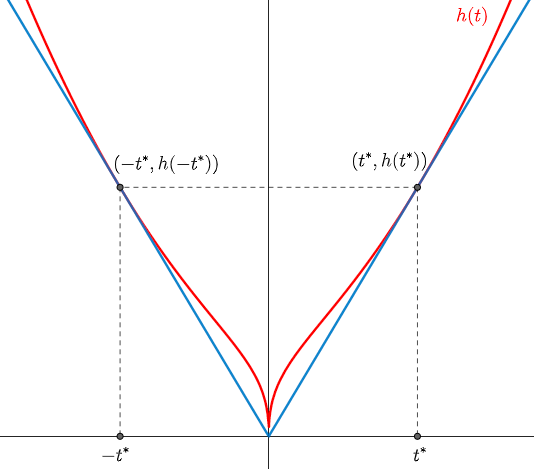
\includegraphics[scale=0.5]{convex.png}
        \begin{tikzpicture}[scale=1]
			 %
				\begin{axis}[
					%domain=-15 :15 ,
					samples=200,
					axis lines=middle,
					ymax=1,
					ymin=0,
					xmax=1,
					xmin=-1,
					%y post scale=-1.5,
					xtick={-2,-0.5,0,0.5,2},
					yticklabels={},%{-1,0,1},
					xticklabels={},%{-2,-0.5,0,0.5,2},
					axis line style={gray},
					%anchor=origin, % Shift the axis so its origin is at (0,0)   
					%rotate around={90:(current axis.origin)}, % Rotate around the origin
					]
					\addplot[color=red, thick, domain=-1:1 ] {0.5*x^2+0.5*abs(x)^(0.5)};
					\addplot[color=blue, dashed,thick, domain=-3:-0.6300 ] {0.5*x^2+0.5*abs(x)^(0.5)};
					\addplot[color=blue, dashed,thick, domain=0.6300:3 ] {0.5*x^2+0.5*abs(x)^(0.5)};
					\addplot[color=blue, dashed,thick, domain=-0.6300:0.6300 ] {0.9449*abs(x)};

					%\addplot[color=blue, thick, domain=-2:-1.108 ] {1.2*x-0.7*abs(x)^(-0.5)};
					 \node [draw=black,anchor=center] at (axis cs: 2.4,-2.5) {
					 $
					 \begin{array}{l}
					  %{\color{red} -\tilde\Phi_0}\\
					 %
					  {\color{red}-P_{[u_a,u_b]}}{\color{blue}\tilde\Phi_q, \quad \text{q=1/2}}\
					 \end{array}
					 $
					 %
					 };
					 \node [anchor=center] at (axis cs: -0.3,4.5) {
					 $p$};
					 \node [anchor=center] at (axis cs: -0.1,-0.1) {
					 $u^*$};
					 \node [anchor=center] at (axis cs: -0.3,-2.3) {
					 $-u^*$};
					 \node [anchor=center] at (axis cs: 2.4,0.5) {
					 $\bar u$};
				\end{axis}				
			\end{tikzpicture}	
        \caption{Graph of $h$ (red line) and its bi-conjugate $h^{**}$ (dashed blue)}
        \label{convex_example}
    \end{figure}  


%    We point out that, for each $u\in L^2(\om)$, the integral $\int_{\om}h(u)\; dx$ corresponds to the terms involved with $u$ explicit in the cost function of \eqref{P}. So, since $h^{**}$ corresponds, in its one dimensional version, a convexification of the non convex part present in \eqref{P}, obviously in its one dimensional form, we call the following problem:

 \begin{lemma}\label{l:h_integrable}
    The biconjugate $h^{**}$ given in Lemma \ref{l:biconjugate}, defines a continuous nonlinearity from $L^2(\Omega)$ into $L^1(\Omega)$.
\end{lemma}
\begin{proof}
    Let us verify that $h^{**}$ satisfies condition (C)  and the growth condition (2.2) in \cite[p.g. 16]{ambrosetti}. Then, \cite[Theorem 2.2]{ambrosetti} implies that $h^{**}$ defines a continuous Nemitski operator from $L^2(\Omega)$ into $L^1(\Omega)$. First, according to  \eqref{biconjugate}, we notice that for $|t|<t^*$ it follows that
    \[
    |h^{**}(t)|<r^*t^*,
    \]
    and for $|t|\ge t^*$ we have that $|t|^{2-q}\ge(t^{**})^{2-q}=2\frac{\beta}{\alpha}(1-q)>\frac{\beta}{\alpha}(1-q)$. This implies that 
    \[
    |t|^{2}>\frac{\beta}{\alpha}(1-q)|t|^q.
    \]
    Finally, we have that for all $t\in \mathbb{R}$ 
    \[
    |h^{**}(t)|<r^*t^*+\left (\frac{\alpha}{2}+\frac{\alpha}{\beta(1-q)}\right)|t|^2.
    \]

\end{proof}  
 
Thanks to  Lemma \ref{l:h_integrable}, we introduce the convex optimal control problem as the convex relaxation of $(P_\lambda)$: 
    \begin{equation}\label{convex}\tag{$P^C_{\lambda}$}
    \begin{cases}
    \displaystyle\min_{(u,y)\in L^2(\om)\times H^1(\Omega)} \; J^C(y,u):=\frac{1}{2}\norm{y-y_d}^2_{L^2(\om)}+\int_{\Omega}h^{**}(u)\; dx\\
    \mbox{subject to:}\\
    Ay(x)=u(x), \phantom{aaaaa} \mbox{in } \om,\\
    \partial_{\nu}y(x)=0, \phantom{aaaaaaaaaaaaa} \mbox{over } \Gamma,\\    
    y_a\le y(x)+\lambda u(x)\le y_b,\phantom{a} \mbox{almost all }x\in \Omega
    \end{cases}
    \end{equation}
    
   
Notice that this problem has a  cost function that is convex, continuous and bounded-from-below. These properties allow us to apply the direct method.
\begin{lemma}
       Problem \eqref{convex} has a solution in $L^2(\om)$.
   \end{lemma}
   \begin{proof}
       % Define $J(u)=\frac{1}{2}\norm{Ru-y_d}_{L^2(\Omega)}^2+ \int_{\Omega}h^{**}(u)\, dx$. 
       Let $\{(u_k,y_k)\}_{k\in \mathbb{N}}\in L^2(\Omega)\times H^1(\Omega)$ a minimizing and admissible sequence for \eqref{convex}, i.e., for each $k$, $y_k \in H^1(\Omega)$ satisfies the state equation with associate control $u_k \in L^2(\om)$. Moreover, the pair $(u_k,y_k)$ satisfies the mixed-constraints:
    \[
    y_a\le y_k(x)+\lambda u_{k}(x)\le y_b,
    \]

The minimizing sequence $\{(u_k,y_k)\}_{k\in \mathbb{N}}$ is bounded. Indeed, $\{u_k\}_{k\in \mathbb{N}}$ is bounded in $L^2(\Omega)$  due to the presence of the Tikhonov penalizer $\frac{\alpha}{2}\|u\|_{L^2(\Omega)}^2$ in the cost function, with $\alpha>0$. Moreover, thanks to the estimate \eqref{continuity_bilinear} we have that: $$ \norm{y_k}_{H^1(\Omega)}\leq c_A \norm{u_k}_{L^2(\Omega)},$$
which shows that $\{y_k\}_{k\in \mathbb{N}}$ is bounded in $H^1(\om)$. %Thereby, the sequence $(y_k,u_k)_{k\in\mathbb{N}}$ forms a bounded sequence in the Hilbert space $L^2(\Omega)\times H^1(\Omega)$. 
Therefore, there exists  a subsequence (without renaming) of $(y_k,u_k)_{k\in\mathbb{N}}$  such that $(y_{k},u_{k})\rightharpoonup (\hat{y},\hat{u})$ in $H^1(\Omega)\times L^2(\Omega)$. Moreover, it is known by the compact embedding $H^1(\Omega) \hookrightarrow \hookrightarrow L^2(\Omega)$ that the weakly convergence of $y_k$ to $\hat{y}$ in $H^1(\Omega)$ implies that $y_{k}\to y$ strongly in $L^2(\Omega)$ as $k\to \infty$. Thus,  we can pass to the limit $k\to \infty$ in the weak formulation in \eqref{continuity_bilinear}, obtaining that
    \[
        a(\hat y, v)=\lim_{k\to\infty}a(y_k,v) = \lim_{k\to\infty}(u_k,v)_{L^2(\Omega)}=(\hat u,v),\quad \forall v \in H^1(\Omega),
    \]
implying that the weak limit $(\hat y,\hat u)$ satisfies the state equation. 

On the other hand, the weak convergence  $u_k \rightharpoonup \hat u$, and the strong convergence $y_k \to \hat y$ in $L^2(\Omega)$ imply that, for any $\lambda>0$, $y_k+\lambda u_k\rightharpoonup \hat{y}+\lambda\hat{u}$ weakly in $L^2(\om)$. In view that 
 the set 
\[
    U_{ad}:=\{v\in L^2(\om ):y_a\le u(x)\le y_b \mbox{ almost all }x\in \om\}
\]
is a closed and convex set in $ L^2(\Omega)$ and thus weakly closed in $L^2(\om)$, then $\hat{y}+\lambda\hat{u}\in U_{ad}$. This shows that the limit points $(\hat{u},\hat{y})$ are also feasible for the problem. 

Let us denote $\hat{J}=\inf_{(y,u)} J^{C}(y,u)$. The convexity and continuity of $J$ imply that $J$ is a weakly lower semicontinous functional. Therefore,
       \[
       \hat{J}=\lim_{n\to \infty}J^{C}(y_{k_n},u_{k_n})\ge \liminf_{n\to \infty}J(y_{k_n},u_{k_n})\ge J^{C}(\hat{y},\hat{u}),
       \]
       thus $(\hat{y},\hat{u})$ minimizes $J$. %Since  $\hat{y}=R\hat{u}$ we have checked that the pair $(\hat{u},\hat{y})$ is a solution for \eqref{convex}.
   \end{proof}\\

\subsection{Optimality conditions for the relaxed problem $(P^C_\lambda)$}
Analogous to smooth optimal control problems governed by partial differential equations, the role of the adjoint state to express first-order information is required. Let us denote the adjoint state associated to a $y \in H^1(\om)$  by $\phi$, solution of the adjoint state equation:
\[
\begin{cases}
A^* {\phi}=y-y_d, &\mbox{ in }\Omega,\\
\partial_{\nu} \phi=0, &\mbox{ on }\Gamma.
\end{cases}
\]
By the same arguments of the state equation \eqref{weak_adjoint_formulation}, this problem has a unique solution $\phi \in H^1(\om)$. Moreover, it is clear that $\phi=S^*(y-y_d)$ for the adjoint operator $S^*$ of $S$ defined through the analysis of equations \eqref{continuity_adjoint_bilinear} and \eqref{weak_adjoint_formulation}.

Using the compact embedding $E:H^1(\Omega) \to L^2(\Omega)$ we define $R: L^2(\om) \to  L^2(\om)$ by $R=ES$. Now, since  $R$ is invertible we introduce the Fredholm operator  
$$B_{\lambda}:L^{2}(\om)\to L^{2}(\om), \qquad \text{by} \qquad B_\lambda =(R+ \lambda I)^{-1},$$ 
\begin{equation} \label{eq:B_Lamb1}   
B_{\lambda}v=B_{\lambda}(y+\lambda u)=(\lambda I+R)^{-1}(\lambda I+R)u=u.
\end{equation}
Furthermore, $R$ is a compact operator Therefore $B_\lambda$ is a Fredholm operator that has only countable many eigenvalues accumulating at $0$. 

Following \cite{meyer1}, we make the following change of variable:  $v=y+\lambda u$. Thus, by using \eqref{eq:B_Lamb1} the problem $(P^C_\lambda)$ can reformulated as a reduced optimization problem with control constraints:
\begin{subequations}\label{eq:reduced}
\begin{align}%\label{reduced}
    &\min_{v\in L^2(\Omega)}\frac{1}{2}\norm{SB_{\lambda}v-y_d}_{L^2(\om)}^2+\int_{\om}h^{**}(B_{\lambda}v), \label{eq:reduced_PClamb} \\
    & \text{ subjec to : } v \in V_{ad}=\{v\in L^2(\om): y_a\le v(x)\le y_b, \text{ almost all }x\in \om\} \label{eq:boxconst_PClamb}.
\end{align}
\end{subequations}


Optimality conditions for problem \eqref{eq:reduced} are obtained by using the Fermat's principle applied to the convex function 
$$F(v)= \frac{1}{2}\norm{SB_{\lambda}v-y_d}_{L^2(\om)}^2+ G(B_\lambda v) + \mathbf{I}_{V_{ad}}(v), \quad \text{with} \quad G(u) = \int_\om h^{**}(u) dx.$$
%. By denoting $\var v$ the optimal solution  i.e. $0 \in \partial F(\bar u)$
Therefore, in view of the the calculus rules for subdifferentials of convex functions,  the solution  $\bar v$ of \eqref{eq:reduced} is characterized by the inclusion: 

\begin{equation}\label{eq:oc_v}
0 \in \partial F (\bar v)= B_\lambda^*S^*(SB_\lambda \bar v -y_d) + B_\lambda^* \partial G(B_\lambda \bar v) + \partial \mathbf{I}_{V_{ad}}(\bar v) \end{equation}

{\color{red}[Todo lo que está en azul, a continuación,  debe estructurarse como un teorema y su demostración, no usar el subíndice $\lambda$ en las variables, ni usar una sucesión $\lambda_n$, solamente concentrarse en el sistema para el problema relajado]}
\begin{theorem}
    Let $\bar{u}\in L^{2}(\Omega)$ an optimal control for problem \eqref{convex}, and $\bar{y}$ its associated optimal state. There exists $\overline{\phi}\in H^1(\Omega)$, $\mu_a, \mu_b, \zeta\in L^2(\Omega)$ such that the following optimal system is full-filled:    \begin{equation}\label{optimality_convex}
        \begin{split}         
        &A\bar{y}=\bar{u}, \hspace{3.5cm} \mbox{in }\Omega\\
        &\partial_{\nu}\bar{y}=0, \hspace{3.45cm} \mbox{on }\Gamma,\\
        &A^*\overline{\phi}=\bar{y}-y_d+\mu_b-\mu_a, \qquad \mbox{in }\Omega,\\
        &\partial_{\nu}\overline{\phi}=0,\hspace{3.5cm}\mbox{on }\Gamma,\\        
        &\overline{\phi}+\zeta+\lambda(\mu_b-\mu_a)=0,\\
        &\mu_a, \mu_b\ge 0,\\
        &\mu_a(\lambda \bar{u}+\bar{y}-y_a)=\mu_b(\lambda \bar{u}+\bar{y}-y_b)=0,\\
        &\zeta(x)=\begin{cases}
            \alpha \bar{u}(x)+\beta q |\bar{u}(x)|^{q-1}\sign(\bar{u}(x)), &|\bar{u}(x)|>t^*,\\
            r^*\sign(\bar{u}(x)), &|\bar{u}(x)|\le t^*, |\bar{u}(x)|\ne 0,\\
            \eta \in [-r^*,r^*],& |\bar{u}(x)|=0.
        \end{cases}  
        \end{split}
    \end{equation}    
\end{theorem}
\begin{proof}
    The mixed constrains present in \eqref{convex} make us to deduce first the optimality system of \eqref{eq:reduced} and then to deduce the system for \eqref{convex} from this one. Details are as follows: let $\overline{v}$ the optimal control for \eqref{eq:reduced}, whose existence can be deduced from the convexity of the cost function in this problem, the structure of the feasible control set, the properties of the linear operators $S$ and $B_{\lambda}$, and following similar steps as in Lemma 4. By Lemma 3 we have that any $\zeta\in \partial G(\overline{v})$ satisfies $ \zeta \in L^2(\Omega)$ and moreover, we can compute it explicit from \eqref{sub_biconjugate}. On the other hand, $\overline{\phi}$ is the solution of the adjoint equation $A^*\overline{\phi}=\bar{y}-y_d$, so $\overline{\phi}\in L^2(\om)$ and therefore $\overline{\phi}+\zeta \in L^2(\Omega)$. Now, define $\mu_a:=[B_{\lambda}^*(\overline{\phi}+\zeta)]_+$ and $\mu_b:=[B_{\lambda}^*(\overline{\phi}+\zeta)]_-$. Accordingly to the the definition of the operator $B_{\lambda}$ and the positive and negative parts of a function, we have that $\mu_a, \mu_b\in L^2(\om)$. Using a well-known result about control problems with box constrains over the optimal control, (see for example \cite{trol}), we have that $\mu_{a}(\overline{v}-y_a)=\mu_b(\overline{v}-y_b)=0$ almost all $x\in \om$, and moreover 
   \[
   \overline{\phi}+\zeta+\mu_b-\mu_a=0,
   \]
   where $\zeta\in \partial G(B_{\lambda}\overline{v})$, and $\overline{v}$ the optimal control for \eqref{eq:reduced}. From here, it is easy to recover the original optimal system for \eqref{convex}, using the the definition of $B_{\lambda}$ and the calculus rules for the convex subdifferentials (see \cite{combettes}). In fact, due to the relation $\bar{u} = B_\lambda \bar v$ and since $\overline{v}$ is an optimal solution for \eqref{eq:reduced}, we deduce that $\bar{u}$ is optimal for \eqref{convex}, and therefore, its associated state $\bar{y}:=R\bar{u}$, is optimal state for \eqref{convex}. Now, the composition of $F$ with a linear operator calculus rule tell us that 
\begin{equation}\label{eq:oc_u}
    0 \in B_\lambda^*(\bar \phi + \partial G(\bar u)) + \mu_b-\mu_a.
\end{equation}
Due to the inverbility of $B_{\lambda}$, \eqref{eq:oc_u} is equivalent to
\[
\bar \phi+\zeta+B^{-*}_{\lambda}(\mu_b-\mu_a)=0.
\]
Using the fact that $\overline{v}=\lambda\bar{u}+\bar{y}$, the complementary conditions $\mu_{a}(\overline{v}-y_a)=\mu_b(\overline{v}-y_b)=0$ are changed to $\mu_a(\lambda\bar{u}+\bar{y}-y_a)=\mu_b(\lambda\bar{u}+\bar{y}-y_b)=0$. Finally, since $B^{-*}_{\lambda}(\mu_b-\mu_a)=\lambda(\mu_b-\mu_a)+R^*(\mu_b-\mu_a)$, the linearity of $R^*$ and the definition of the adjoint state allow us to complete the demonstration.
\end{proof}

\subsection{Existence of solutions for the non convex problem}

The last Theorem provide us candidates for optimal solutions to \eqref{plambda}. The following result allow us to demonstrate that a solution for \eqref{convex}, under suitable conditions chosen from the optimal system \eqref{optimality_convex}, is, in fact, an optimal solution for the original problem. Details are as follows.

\begin{theorem}
    Let $(\bar{y},\bar{u})$ an optimal solution for \eqref{convex} and assume that the set $\om^*:=\{x\in \om: 0<|\bar{u}(x)|<t^*\}$ has zero measure. Then, $(\bar{y},\bar{u})$ is a solution for $\eqref{plambda}$.
\end{theorem}
\begin{proof}
    Pick up any $(y,u)\in H^{1}(\om)\times L^2(\om)$ feasible for \eqref{plambda}. A standard computation show us that
     \begin{equation}\label{eq1:theorem2}
     \begin{split}
        J(y,u)-J(\bar{y},\bar{u})=&(\bar{y}-y_d, R(u-\bar{u}))_{L^2(\Omega)}+\alpha(\bar{u},u-\bar{u})_{L^2(\Omega)}\\
        &+\frac{1}{2}\norm{y-\bar{y}}_{L^2(\om)}^2+\frac{\alpha}{2}\norm{u-\bar{u}}_{L^2(\om)}^2\\
        &+\beta\left(\int_{\Omega}|u(x)|^q\; dx-\int_{\om}|\bar{u}(x)|^q\; dx\right).
        \end{split}
    \end{equation}

    Now, due to the third and fifht equation of \eqref{optimality_convex} we have that
    \begin{align*}
        (\bar{y}-y_d, R(u-\bar{u}))_{L^2(\Omega)}&=(\overline{\phi}, u-\bar{u})_{L^2(\Omega)}-(\mu_b-\mu_a,R(u-\bar{u}))_{L^2(\Omega)}\\
        &=(-\zeta-\lambda(\mu_b-\mu_a),u-\bar{u})_{L^2(\om)}-(\mu_b-\mu_a,R(u-\bar{u}))_{L^2(\Omega)}\\
        &=(-\zeta,u-\bar{u})_{L^2(\om)}-(\mu_b-\mu_a,\lambda(u-\bar{u}))_{L^2(\om)}\\
        &\phantom{=-}-(\mu_b-\mu_a,y-\bar{y})\\
        &=(-\zeta,u-\bar{u})_{L^2(\om)}-(\mu_b-\mu_a,\lambda u+y-\lambda \bar{u}-\bar{y})_{L^2(\om)},
    \end{align*}
  where the third equation above corresponds to the identity $Ru=y$ and $R\bar{u}=\bar{y}$, which is verified since $(y,u)$ is admissible for \eqref{plambda} and $(\bar{y},\bar{u})$ is the solution for \eqref{convex}. Now, suppose that almost all $x\in \om$, $y_a<\lambda u(x)+y(x)<y_b$. Then, due to the complementary contidions in the seventh equation in \eqref{optimality_convex} we have that $\mu_a(x)=\mu_b(x)=0$, so in this subset of $\om$ we have that $(\bar{y}-y_d, R(u-\bar{u}))_{L^2(\Omega)}=(-\zeta,u-\bar{u})_{L^2(\om)}$. Consider now the set of almost all $x\in \om$ such that $\lambda \bar{u}(x)+\bar{y}(x)=y_b$. Then, again by the complementary equations we have that $\mu_a=0$. But, since $(\bar{y},\bar{u})$ is feasible for \eqref{plambda}, we have that $\lambda u(x)+y(x)-y_b\le 0$, so in this subset of $\om$, $(\mu_b-\mu_a,\lambda u+y-\lambda \bar{u}-\bar{y})_{L^2(\om)}\le 0$. Finally, for all $x\in \om$ such that $\lambda \bar{u}(x)+\bar{y}(x)=y_b$, we have that $\mu_b=0$ accordingly the complementary conditions mentioned before. The feasibility of $(y,u)$ again tell us that $\lambda u(x)+y(x)-y_a\ge 0$ so in this set we have again $(\mu_b-\mu_a,\lambda u+y-\lambda \bar{u}-\bar{y})_{L^2(\om)}\le 0$. Therefore, we conclude that for almost all $x\in \om$,
  \[
  (\mu_b-\mu_a,\lambda u+y-\lambda \bar{u}-\bar{y})_{L^2(\om)}\le 0,
  \]
  and therefore
  \[
  (\bar{y}-y_d, R(u-\bar{u}))_{L^2(\Omega)}\ge (-\zeta,u-\bar{u})_{L^2(\om)}.
  \]
  The last inequality show us that \eqref{eq1:theorem2} changes to the relation
  \begin{equation}\label{eq2:theorem2}
     \begin{split}
        J(y,u)-J(\bar{y},\bar{u})\ge&(\alpha\bar{u}-\zeta,u-\bar{u})_{L^2(\Omega)}\\
        &+\frac{1}{2}\norm{y-\bar{y}}_{L^2(\om)}^2+\frac{\alpha}{2}\norm{u-\bar{u}}_{L^2(\om)}^2\\
        &+\beta\left(\int_{\Omega}|u(x)|^q\; dx-\int_{\om}|\bar{u}(x)|\; dx\right).
        \end{split}
    \end{equation}
In order to analyze the sign of the right hand part of \eqref{eq2:theorem2}, we must divide $\om$ into two more sets in addition to $\om^*$: $\om_1^*:=\{x\in \om:|\bar{u}(x)|\ge t^*\}$ and $\om^*_2:=\{x\in\om:\bar{u}(x)=0\}$ and split the inner product and the integrals present in \eqref{eq2:theorem2} into these domains. Now, for almost all $x\in \om_1^*$ we can follow similar arguments presented in \cite{merino-nejer} to show that
\begin{equation}\label{eq3:theorem2}
\begin{split}   
\int_{\om_1^*}(\alpha\bar{u}(x)-\zeta(x))(u(x)-\bar{u}(x))+\beta&\left(|u(x)|^q-|\bar{u}(x)|\right)\; dx\\
&>-q\frac{\alpha}{2}\int_{\om_1}(u(x)-\bar{u}(x))^2\; dx
    \end{split}
\end{equation}
Now, the analysis of sign for the domain $\om_2^*$ is slightly different from the presented in \cite{merino-nejer}. In fact, since $\bar{u}(x)=0$ over $\om_{2}^*$, we also have that
\begin{equation}\label{eq4:theorem2}
\begin{split}   
\int_{\om_2^*}(\alpha\bar{u}(x)&-\zeta(x))(u(x)-\bar{u}(x))+\beta\left(|u(x)|^q-|\bar{u}(x)|^q\right)\; dx\\
&=\int_{\om_2^*}\eta u(x)+\beta |u(x)|^q+\frac{\alpha}{2}|u(x)|^2\; dx-\int_{\om_2^*}\frac{\alpha}{2}|u(x)|^2,
    \end{split}
\end{equation}
where $|\eta|\le r^*$, according to the form of $\zeta$ in \eqref{optimality_convex}. Define the unidimensional function $\varphi(t):=\eta t+\beta|t|^q+\frac{\alpha}{2}|t|^2$ for all $t\in \mathbb{R}$. Notice that 
\[
\varphi(t)=\eta t+h(t).
\]
Now, by \eqref{lemma1:ineq1} we have that $h(t)\ge r^*|t|$ for all $t\in \reals$, so 
\begin{align*}
    \varphi(t)&=\eta t+h(t)\\
                &\ge r^*|t|+\eta t\\
                &|t|(r^*+\eta\sign(t))\ge 0,
\end{align*}
since $\eta\sign(t)\in [-r^*,r^*]$. Therefore, 
\[
\eta u(x)+\beta |u(x)|^q+\frac{\alpha}{2}|u(x)|^2\ge 0,
\]
for all $x\in \om_2^*$, and \eqref{eq4:theorem2} is equivalent to
\begin{equation}\label{eq5:theorem2}
\begin{split}   
\int_{\om_2^*}(\alpha\bar{u}(x)-\zeta(x))(u(x)-\bar{u}(x))+&\beta\left(|u(x)|^q-|\bar{u}(x)|^q\right)\; dx\\
&\ge-\int_{\om_2^*}\frac{\alpha}{2}|u(x)|^2\; dx,
    \end{split}
\end{equation}
Recalling \eqref{eq1:theorem2} and combining \eqref{eq2:theorem2} and \eqref{eq4:theorem2} we have that
\begin{align*}
    J(y,u)-J(\bar{y},\bar{u})&>\frac{\alpha}{2}\norm{u-\bar{u}}_{L^2(\om)}^2-q\frac{\alpha}{2}\int_{\om_1^*}(u(x)-\bar{u}(x))^2\; dx -\int_{\om_2^*}\frac{\alpha}{2}|u(x)|^2\\
    &\phantom{>}+o\left(\norm{u-\bar{u}}_{L^2(\om)}^2\right)+\frac{1}{2}\norm{y-\bar{y}}_{L^2(\om)}^2\\    
    &\ge (1-q)\frac{\alpha}{2}\int_{\om_1^*}(u(x)-\bar{u}(x))^2\; dx\ge 0,
\end{align*}
proving that $(\bar{y},\bar{u})$ is optimal for \eqref{plambda}.
\end{proof}





\section{Difference of convex functions approach for problem \eqref{plambda}}

In this section we derive an optimality system suitable for numerical computation of solutions for \eqref{plambda}. The technique presented in \cite{merino}  allows us to derive an optimality system using DC-programming theory. However,  it is required to approximate  $L^q$-quasinorm penalty by means of a \textit{Huber type regularization} which allow us reformulating the cost function of \eqref{plambda} as the difference of two convex functions. Then, first order necessary conditions for the regularized problem are obtained using the DC-criticality in terms of a optimality system that will be useful to formulate a Newton semismooth algorithm.

\subsection{Difference-of-convex function formulation \eqref{plambda}}

For $q\in ]0, 1[$ and $\gamma>>1$, the following smoothing function of the absolute value where proposed in \cite{merino} to take into account the exponent $q$ :
\[
|t|_{q,\gamma}(t)=\begin{cases}
q\gamma^{\frac{1-q}{q}}|t|^{\frac{1}{q}}, & |t|\le \frac{1}{\gamma},\\ 
|t|-\frac{1-q}{\gamma}, & |t|>\frac{1}{\gamma}.
\end{cases}
\]
defined for all $t\in \mathbb{R}$. Then, for each $u\in L^2(\om)$ we define the mapping
\[
u \mapsto\int_{\om}|u(x)|_{q,\gamma}^q\; dx,
\]
which is a \textit{Huber-type regularization} for the quasi norm $\int_{\om}|u|^q\; dx$ present in \eqref{P}.
The regularized  optimal control problem reads:
\begin{equation}\tag{$P^\gamma_{\lambda}$} \label{phuber}
    \begin{cases}
    \displaystyle\min_{(y,u)\in H^1(\om)\times BV(\om)} \frac{1}{2}\norm{y-y_d}^2_{L^2(\om)}+\frac{\alpha}{2}\norm{u}^2_{L^2(\om)}+\beta\int_{\om}|u(x)|_{\gamma,q}^q \,dx\\
    \mbox{subject to:}\\
    Ay(x)=u(x), \phantom{aaaa} \mbox{in } \om,\\
    \partial_{\nu}y(x)=0, \phantom{aaaaaaaaaaaa} \mbox{on } \Gamma,\\
   y_a\le\lambda u(x)+y(x)\le y_b, \phantom{aaa} \mbox{a.e in }\om 
    \end{cases}
\end{equation}
As same as the previous Section, if we define the artificial control $v=(\lambda I+R)u$, for any $u\in L^2(\om)$, and if we introduce the indicator function (see Section 2), \eqref{phuber} can be reformulated as 
\[
	\begin{cases}
		\displaystyle \min_{v\in L^{2}(\om)} \qquad  \frac{1}{2}\norm{S	B_{\lambda}v-y_d}_{L^2(\om)}^2+\frac{\alpha}{2}\norm{	B_{\lambda}v}_{L^2(\om)}^2+\beta\int_{\om}|(B_\lambda v)(x)|_{\gamma,q}^q \,dx+\mathbf{I}_{V_{ad}}(v),
		\end{cases}
\]
where $ V_{ad}:=\{v\in L^2(\om): y_a\le v(x)\le y_b, \mbox{ a.e }x\in K\subset\subset\om \}$. Now, for every $v\in L^2(\om)$ we set 
$$\kappa_\gamma = q^{q}\gamma^{1-q},$$
and define the functions
\begin{equation}\label{convexI}
	G(v):=\frac{1}{2}\norm{S	B_{\lambda}v-y_d}_{L^2(\om)}^2+\frac{\alpha}{2}\norm{	B_{\lambda}v}_{L^2(\om)}^2+\beta\kappa_{\gamma}\norm{B_{\lambda}v}_{L^{1}(\om)}+\mathbf{I}_{V_{ad}}(v),
\end{equation}
and
\begin{equation}\label{convexII}
	H(v):=\beta \l(\kappa_{\gamma}\norm{B_{\lambda}v}_{L^{1}(\om)}-\beta\int_{\om}|(B_\lambda v)(x)|_{\gamma,q}^q \,dx\r).
\end{equation}


{\color{red}
\begin{lemma}
    Let $H: L^2(\om) \to \reals$ be the function defined  in \eqref{convexII}. Then, $H$ is G\^ateaux differentiable and the corresponding derivative is given by
    \begin{equation}
        (B^*_\lambda w,\cdot)_{L^2(\om)}, \quad \text{where }\quad 
        w = 
         \begin{cases}
            \kappa_{\gamma}-q\l(|B_\lambda v(x)|+\dfrac{q-1}{\gamma}\r)^{q-1}\sign(t), & \mbox{if }|B_\lambda v(x)|\ge \frac{1}{\gamma},\\
            0, &\mbox{otherwise},
        \end{cases}
    \end{equation}
\end{lemma}
\begin{proof}
\end{proof}
Moreover, it was proved in \cite{} that $H$ is G\^ateaux differentiable from $L^2(\om)$ into $\real$ and its derivative at $v\in L^2(\om)$, is given by
 \[
        t\mapsto \kappa_{\gamma}|t|-h_{q,\gamma}(t),
    \]
is Gâteaux differentiable (see Lemma 6 of \cite{merino}), with derivate
 \begin{equation}\label{j}
        j(t)=\begin{cases}
            \kappa_{\gamma}-q\l(|t|+\dfrac{q-1}{\gamma}\r)^{q-1}\sign(t), & \mbox{if }|t|\ge \frac{1}{\gamma},\\
            0, &\mbox{if not},
        \end{cases}
    \end{equation}
    and moreover, from the linearity and invertibility of $B_{\lambda}$ for small enought $\lambda$ and the Gâteaux differentiability of $h_{q,\gamma}$, we get the Gâteaux differentiability of $G(B_{\lambda}v)$ for each $v\in V_{ad}$.\\
}

% Previous the deduction of the optimal system for \eqref{phuber}, we present some results. The next result allow us to well define the subdifferential of $\int_{\om} h^{**}(u)\; dx$ for each $u\in L^2(\om)$.



Observe that $H$ and $G$ defined in \eqref{convexI} and \eqref{convexII} respectively, are convex functions. Indeed, $G$ is composed of the sum of norms and the indicator function, each applied through affine-linear continuous operators. On the other hand, convexity for $H$ follows from \cite[Lemma 5]{merino}) and the fact that $H$ involves the same function composed with the continuous linear operator $B_\lambda$. Hence,  problem \eqref{1} can be expressed as the minimization of the difference of the convex functions $G$ and $H$:
\begin{equation}\label{1}
    	\min_{v\in L^2(\om)} G(v)-H(v).
\end{equation}

From the theory of Difference of Convex functions (DC-theory, see for example \cite{dihn, merino})  we know that if $\overline{v}$ is a solution for problem \eqref{1}, then $\bar v$ satisfies the inclusion 
\begin{equation}\label{opt}
    \partial H(\overline{v})\subset\partial G(\overline{v}),
\end{equation}

We rely in \eqref{opt} to derive an alternative optimality system. First, let us characterize the subdifferentials of $H$ and $G$. For this purpose, consider the regular part of $G$:
\[
	f(v):=\frac{1}{2}\norm{S	B_{\lambda}v-y_d}_{L^2(\om)}^2+\frac{\alpha}{2}\norm{	B_{\lambda}v}_{L^2(\om)}^2,
\]
 which is a quadratiq functional in $L^2(\om)$, thus $f$ is Fréchet differentiable and its derivative is computed by
\[\nabla f(\overline{v})=B_{\lambda}^*(\overline{\phi}+\alpha B_{\lambda}\overline{v}) \in L^2(\om).
\]
and $\overline{\phi}$ the adjoint state solution to the equation {\color{red} usar referencia anterior para esta equación}
\[
\begin{cases}
A^*\phi=y-y_{d}, &\mbox{in }\om\\
\partial_{\nu}\phi=0,&\mbox{over }\Gamma
\end{cases}
\]

The nonsmooth part of $G$ is given by the $L^1(\om)$-norm, whose subdiferential has elements of the form
\begin{equation}\label{zeta}
	\zeta(x)=\begin{cases}
		\{1\}, & \mbox{if }  B_{\lambda}v(x)>0,\\
		\{-1\}, & \mbox{if } B_{\lambda}v(x)<0\\
		 [-1,1], &\mbox{if }  B_{\lambda}v(x)=0,
	\end{cases}
\end{equation}
for almost all $x\in \om$. Then, from \eqref{opt} and the theory of convex analysis (see for example \cite{rock}) we deduce that if $\overline{v}$ is a solution of \eqref{opt} {\color{red}with state $\bar y$ solution of  equation \eqref{}}, there exists $\overline{w}\in L^2(\om)$, {\color{red} $\overline{\phi}\in H^1(\om)$ solution of the adjoint equation \eqref{} }, $\zeta\in L^{\infty}(\om)$ y $\theta \in N_{V_{ad}}$ such that     
     \begin{equation}\label{gradiente1}
         \beta B_{\lambda}^*\overline{w}=B_{\lambda}^*(\overline{\phi}+\alpha B_{\lambda}\overline{v})+\beta\kappa_{\gamma}B_{\lambda}^*\zeta+\theta,
     \end{equation}

Now, from the characterization of the normal cones presented, for example in \cite{rock}, we can deduce the following.
\begin{theorem} 
	If $\overline{v}$ is a solution for \eqref{opt}, then there exists $\bar{y}\in H^1(\om)$, $\overline{w}\in L^2(\om)$, $\overline{\phi}\in H^1(\om)$, $\zeta\in L^\infty(\om)$ such that the following optimal conditions are full-filled
	\begin{equation}\label{optii1}
    \begin{split}
	&A\bar{y}=B_{\lambda}\overline{v}, \\
	&\partial_{\nu} y=0, \\
	&A^*\overline{\phi}+\bar{y}-y_d=0,\\
	&\partial_{\nu}\overline{\phi}=0,\\
	&(B_{
	\lambda}^*(\overline{\phi}+\alpha B_{\lambda}\overline{v}+\beta( \kappa_{\gamma}\zeta-w)),v-\overline{v})_{L^2(\om)}\ge 0, \;\forall v \in V_{ad},\\
	&\zeta(x)=\begin{cases}
		\{1\}, & \mbox{if }  B_{\lambda}v(x)>0,\\
		\{-1\}, & \mbox{if } B_{\lambda}v(x)<0\\
		 [-1,1], &\mbox{if }  B_{\lambda}v(x)=0,
	\end{cases}\\
	&w-j(B_{\lambda}\overline{v})=0.
\end{split}
\end{equation}
\end{theorem}

\begin{proof}
 It is a well-know fact that, if $Y$ is a convex cone, then its normal cone $N_{Y}$ is characterized as
\[
    N_{Y}(x)=\partial \mathbf{I}_{Y}(x)=\{x^*\in X^*:\langle x^*, \tilde{x}-x\rangle_{X^*,X}\le 0,  \mbox{ for all }\tilde{x}\in Y\}.
\]
See, for example \cite{rock}. So, using the Riesz representative of $B_{
	\lambda}^*(\overline{\phi}+\alpha B_{\lambda}\overline{v}+\beta( \kappa_{\gamma}\zeta-w))$ and using the same notation for it, then the gradient equation \eqref{gradiente1} is converted into the presented form in the optimal system presented above.
\end{proof}\\

The next theorem allow us to rewrite the last optimal system in terms of the originals state and control $y, u$, and introducing two $L^{2}(\om)$ Lagrange multipliers which they allow us to rewrite the gradient inequality presented above.

\begin{lemma}
Let $\bar{u}\in L^2(\om)$ the optimal control state of \eqref{plambda}. Then, there exists $\bar{y}, \overline{\phi}\in H^1(\om)$, $\mu_a,\mu_b, \overline{w}\in L^2(\om)$, $\zeta\in L^{\infty}(\om)$ such that the following KKT system is full filled:
%\newpage
\begin{equation}\label{opti3}
\begin{split}
	&A \overline y=\bar{u}, \qquad\qquad\qquad\qquad \; \mbox{in }\om,\\
	&\partial_{\nu} y=0, \qquad\qquad\qquad\qquad\qquad \mbox{over }\Gamma,\\
	&A^*\overline{\phi}+\bar{y}-y_d-\mu_{b}+\mu_{a}=0,\quad \;\;\mbox{in }\om,\\
	&\partial_{\nu}\overline{\phi}=0,\qquad\qquad\qquad\qquad\qquad \mbox{over }\Gamma,\\
	&\overline{\phi}+\alpha \bar{u}+\beta( \kappa_{\gamma}\zeta-\overline{w})+\lambda( \mu_b- \mu_a)=0,\\
	&\mu_{a}, \mu_{b}\ge 0,\\
	&\mu_{a}(\lambda\bar{u}+\bar{y}-y_a)=\mu_{b}(B_\lambda\bar{u}+\bar{y}-y_b)=0,\\
    &\overline{w}-j(\lambda u+y)=0
\end{split}
\end{equation}
and
\[
\zeta(x)=\begin{cases}
		1, & \mbox{a.a. }x\in \om \mbox{ such that } \bar{u}(x)>0,\\
		-1, & \mbox{a.a. }x\in \om \mbox{ such that } \bar{u}(x)<0,\\
		\mu \in [-1,1], &\mbox{a.a. }x\in \om \mbox{ such that } \bar{u}
  \end{cases}
\]
\end{lemma}

\begin{proof}
    Calling 
    \[
    \mu_a=[B_{\lambda}^*(\overline{\phi}+\alpha B_{\lambda}\overline{v}+\beta\kappa_{\gamma}\zeta-w)]_{+},\qquad
    \mu_b=[B_{\lambda}^*(\overline{\phi}+\alpha B_{\lambda}\overline{v}+\beta\kappa_{\gamma}\zeta-w)]_{-}, 
\]
it can be followed similar arguments used in Lemma 4 to prove the non negativity and regularity of multipliers $\mu_a, \mu_b$, as well as the complementary conditions that must be satisfied. Finally, if $\overline{v}$ is the solution of \eqref{plambda}, and since $B_{\lambda}\overline{v}=\lambda\bar{y}+\bar{u}$, we can replace all $B_{\lambda}\overline{v}$ terms in \eqref{optii1} with  $B_{\lambda}\overline{v}=\lambda\bar{y}+\bar{u}$, concluding the result. 
\end{proof}


\section{DC Algorithm and DC-Semismooth Newton method}

In this section we propose a numerical solution scheme based on Semi-smooth Newton algorithm (\cite{merino1, ulbrich}). First we define two funtions $C_1:L^2(\om)\times H^{1}(\om)\times L^2(\om)\to L^2(\om)$ and $C_2:L^2(\om)\times L^{\infty}(\om)\to L^2(\om)$, defined as
\[
    C_{1}(\mu,y,u)=\mu-\max(0,c_1(\lambda u+y-y_b)+\mu)+\min(0,c_1(\lambda u+y-y_a)+\mu),
\]
and
\[
C_{2}(u.\zeta)=u-\max(0,u+c_2\kappa_{\gamma}\beta(\zeta-1))-\min(0,u+c_2\kappa_{\gamma}\beta(\zeta+1)).
\]
with these two functions, we can easily verify that the optimal system \eqref{opti3} can be rewrite as

\begin{subequations}\label{1.6}
\begin{align}
    &E\bar{y}-\bar{u}=0,\subtag{a}\\
    &E^*\overline{\phi}-\bar{y}+y_d+\mu=0,\subtag{b}\\
    &\overline{\phi}+\alpha \bar{u}+\beta (\kappa_{\gamma}\zeta-w)+\lambda \mu=0,\subtag{c}\\
    &C_1(u,y,\mu)=0,\subtag{d}\\
    &C_2(u,\zeta)=0,\subtag{e}\\
    &w-j(u)=0,\subtag{f}
\end{align}
\end{subequations}
where $E$ denotes the differential operator associated to the P.D.E that rules the optimal control problem. The following result proves that the left hand sides of \eqref{1.6} can define a semi smooth function (see \cite{ulbrich}).

\begin{lemma}
The function $j$ introduced in \eqref{j} defines a continuous Nemitski  operator from $L^2(\om)$ to $L^2(\om)$.
\end{lemma}

\begin{proof}
Clearly, the function $j$ is a continuous function over $\reals$. Now, if $|t|\le \frac{1}{\gamma}$, $j(t)=0$, so for all constants $a,b>0$ we have $j(t)<a+b|t|$. Suppose that $|t|>\frac{1}{\gamma}$. Then we have
\[
    |j(t)|\le \kappa_{\gamma} +q\l||t|+\frac{q-1}{\gamma}\r|^{q-1}.
\]
Now,
\[
|t|>\frac{1}{\gamma}\Rightarrow |t|+\frac{q-1}{\gamma}>\frac{q}{\gamma}
\]
and since $\gamma>1>q$, we have
\[
    \l(|t|+\frac{q-1}{\gamma}\r)^{1-q}<\l(\frac{q}{\gamma}\r)^{1-q}.
\]
This implies that
\[
|j(t)|<\kappa_{\gamma}+q\l(\frac{q}{\gamma}\r)^{1-q}.
\]
If we define $a=\kappa_{\gamma}+q\l(\frac{q}{\gamma}\r)^{1-q}$, then, clearly
\[
|j(t)|\le a+|t|.
\]
Therefore, the conditions (C) and 2.2 established for continuous Nemintski operators in \cite{ambrosetti} are full-filled, and our result follows from Theorem 2.2 in \cite{ambrosetti}. 
\end{proof}




\begin{theorem}
\normalfont
    Let $E=H^1(\om)\times L^{2}(\om)\times L^{2}(\om)\times L^{2}(\om)\times L^{\infty}(\om)\times L^{2}(\om)$ and $\mathcal{F}: E\to E$ a function with variables $\bar{y},\bar{u},\overline{\phi},\mu,\zeta,w$ defined by the left hand sides of \eqref{1.6}. Then, $\mathcal{F}$ is semi smooth
\end{theorem}
\begin{proof}
For each $u \in L^2(\om)$, define $Tu=S^*(S(u)-y_d)$. Then, we have $\bar{y}=S\bar{u}$, $\overline{\phi}=T\bar{u}$ and $w=j(u)$. from equation c in \eqref{1.6}, it follows that
\[
    \kappa_{\gamma}\beta\zeta=\beta j(u)-\lambda \mu-T\bar{u}-\alpha\bar{u}.
\]
Define 
\[
    \mathcal{F}_1(u,\mu)=\mu-\max(0,c_1(\lambda u+Su-y_b)+\mu)-\min(0,c_1(\lambda u+Su-y_a)+\mu),
\]
\begin{align*}
    \mathcal{F}_2(u,\mu)=&u-\max(0,u+c_2(\beta j(u)-\lambda\mu-Tu-\alpha u-\kappa_{\gamma}\beta))\\
    &-\min(0,u+c_2(\beta j(u)-\lambda\mu-Tu-\alpha u+\kappa_{\gamma}\beta)),
\end{align*}
so $\mathcal{F}(\cdot)=0$ is equivalent to $\mathcal{F}_1(\cdot)=0$ and $\mathcal{F}_2(\cdot)=0$. If we proof that both $\mathcal{F}_1$ and $   \mathcal{F}_2$ are semi smooth, then we can conclude the semi smoothnes of $\mathcal{F}$.


If $c_1=\frac{1}{\lambda}$ we have that
\[
    \mathcal{F}_1(u,\mu)=\mu-\max\l(0,u+\frac{1}{\lambda}Su-\frac{1}{\lambda} y_b+\mu\r)-\min\l(0,u+\frac{1}{\lambda}Su-\frac{1}{\lambda}y_a+\mu\r),
\]
otherwise, if  $c_2=\frac{1}{\alpha}$, we have that
\begin{align*}
    \mathcal{F}_2(u,\mu)=&u-\frac{\beta}{\alpha}\bigg[\max\l(0,j(u)-\frac{\lambda }{\beta}\mu-\frac{1}{\beta}Tu-\kappa_{\gamma}\r)\\
    &-\min\l(0,j(u)-\frac{\lambda }{\beta}\mu-\frac{1}{\beta}Tu+\kappa_{\gamma}\r)\bigg].
\end{align*}
Now, notice that $\mathcal{F}_1$ has the term $M(u,\mu)=u+\frac{1}{\lambda}Su+\mu+c$, which $c$ a constant that could be $-\frac{1}{\lambda}y_a$ or $-\frac{1}{\lambda}y_b$. Since $S$ is a continuous linear operator, clearly $M$ is Fréchet differentiable for any $(u,\mu)\in L^2(\om)^2$. Finally, is a well-known fact that $\max(0,\cdot)$ and $\min(0,\cdot)$ are semi smooth functions are (see for example \cite{delosreyes} o \cite{ito-kunish}). Moreover, the composition of a Fréchet differentiable function with a semi smooth function results in a semi smoot function, proving that $\mathcal{F}_1$ is semi smooth. A similar analysis can be done for proving that $\mathcal{F}_2$ is also a semi smooth function. 
\end{proof}\\

We know (see for example\cite{ulbrich, meyer1, stadler}) that the Semi-smooth Newton type methods are useful for the numerical resolution of the equation
\begin{equation}\label{SSN}
     \mathcal{F}(x)=0,
\end{equation}   

especially when $\mathcal{F}$ is a semi-smooth function. The main idea of the method is the following: given $x^k$, $k\in \mathbb{N}$, the next iteration of SSN method (semi-smooth Newton method) $x^{k+1}$ must satisfies the equation
\[
F(x^k)+\mathcal{G}(x^k)(x^{k+1}-x^k)=0,
\]
where $\mathcal{G}$ denotes the generalized derivate of $\mathcal{F}$. In our case, the generalized derivate has the form 
\begin{equation}
    \mathcal{G}(p)=\begin{pmatrix}
    E               &0      &   -I                  &0                       &0                                           &0\\
    -I              &E      &   0                   &I                       &0                                           &0\\
    0               &I      & \alpha I              &\lambda I               &\beta\kappa_{\gamma}I                       &-\beta I\\
    \chi_{A}        &0      & \lambda(\chi_{A})     &c_1\lambda(I-\chi_{A})    &0                                           &0\\
    0               &0      &   I-\chi_{\tilde{A}}  &0                       &-c_2\kappa_{\gamma}\beta(\chi_{\tilde{A}})    &0\\
    0               &0      &   j'(u_k)             &0                       &   0                                        &-I
    \end{pmatrix}
\end{equation}

with 
\[
    A_1=\{x: c_1(\lambda u+y-y_b)+\mu\ge 0\}, A_2=\{x: c_1(\lambda u+y-y_a)+\mu \le 0\}, A=A_1\cup A_2,
\]
\[
    A_3=\{x:u+c\kappa_{\gamma}\beta(\zeta-1)\ge 0\},  A_4=\{x:u+c\kappa_{\gamma}\beta(\zeta+1)\le 0\},  \tilde{A}=A_3\cup A_4.
\]
Our semi-smooth algorithm is based over similar models proposed, for example in \cite{ulbrich, stadler, meyer1} and many other literature steps. Specifically, the algorithm used in this paper is summarized as follows:  \\

\textbf{Algorithm 1}
\begin{enumerate}
    \item 
    Take $\epsilon>0$, a initial point $p_0=(\bar{y}_0,\overline{\phi}_0,\bar{u}_0,\overline{\mu},\overline{\zeta}_0,\overline{w}_0)$ sufficiently close to the solution of \eqref{SSN} $k=0$ and $\delta_{k}$ appropriately chosen for checking the condition $\norm{d_k}>\epsilon$.    
    \item
       While $\norm{\delta_{p_k}}\ge \epsilon$:
        \begin{enumerate}
            \item 
            Compute $F(x_k)$, $F'(p_k)$ and find $\delta_{p_{k}}$ from the system
            \[
                F'(p_k)\delta_{p_{k}}=-F(p_k)
            \]
            \item
                Take
                \[
                    p_{k+1}=p_k+\delta_{p_k}
                \]
            \item
                Set $\delta_{p_{k+1}}=p_{k+1}-p_{k}$ and compute $\norm{\delta_{p_{k+1}}}$. 
            \end{enumerate}
        \item
        If $\norm{\delta_{p_{k+1}}}\ge \epsilon$, then go to step 2, setting $k=k+1$.  Otherwise, stop the algorithm and take $p_{k+1}$ as the solution for \eqref{SSN}.
\end{enumerate}

The stopping criteria is based on the next argument: since we expect that the the sequence of $(p_n)$ satisfies $\lim_{k\to\infty}\mathcal{F}(p_k)=0$,
the residual $\delta_{p_{n}}$ should tends to zero as $k\to \infty$. The following theorem allow us to expect the convergence of our algorithm to a solution for \eqref{SSN}.

\begin{theorem}
    The algorthim 1 converges to the solution of problem  if $x^0$ is sufficiently close to this solution  
\end{theorem}

\begin{proof}
    We know that $\mathcal{F}$ is a semi-smooth function, so, by Theorem 9 of \cite{stadler}, it is sufficient to prove that $\mathcal{G}$ has a bounded inverse. The inversibility of $\mathcal{G}$ follows from the following facts: first of all, the elliptic operator used in out problem admitis for each $z\in L^2(\om)$ a unique $\overline{\varphi}\in H^1(\om)$ such that $E\varphi=z$. The same holds for $E^*$. Finally, the dependence of the multipliers $\mu, \xi$, as same as the adjoint state, only of the optimal control and state for \eqref{P} follows the fact that there exist only one solution for the equation 
    \[
    \mathcal{G}(X)=Y,
    \]
    where $X,Y\in E$, and $E$ defined as in Theorem 7, and therefore $\mathcal{G}$ is invertible. Finally, the continuity of $E$ and $E^*$, plus the structure of the active sets follows by the Bounded Inverse Theorem that $\mathcal{G}^{-1}$ is bounded, and thereby the Newton semi-smooth method will converge to a solution of the problem.    
\end{proof}


\section{Numerical results}

The optimal control problem that we consider for testing our results is the following: setting $\om=[0,1]^2$, we formulate the problem:

\begin{equation}
    \begin{cases}
    \displaystyle\min_{(y,u)\in H^1(\om)\times L^2(\om)}\; \frac{1}{2}\norm{y-y_d}^2_{L^2(\om)}+\frac{\alpha}{2}\norm{u}^2_{L^2(\om)}+\beta \int_{\om} |u|^{q}\; dx\\
    \mbox{subject to:}\\
    -\Delta y+y=u, \phantom{aaa} \mbox{in } \om,\\
    \partial_{\nu}y(x)=0, \phantom{aaaaa} \mbox{over } \Gamma,\\    
    -1\le y(x)\le 0.2 ,
    \end{cases}
\end{equation}
where 
\[
    y_d(x_1,x_2)=\left(x_1-\frac{1}{2}\right)^2+\left(x_2-\frac{1}{2}\right)^2,
\]
for all $(x_1,x_2)\in [0,1]^2$. For the discretization of the domain and the numerical approximation of the integrals we use a finite difference scheme: using the standar partition of the domain into $n^2$ equidistant nodes $(x_1^i,x_2^j)$ for $i,j=1,\cdots,n$, with $x_1^i=\frac{i}{n+1}$ and $x_2^j=\frac{j}{n+1}$.\\

Setting $h=\frac{1}{n+1}$, we use the following midpoint rule for calculating the double integrals that appear in the problem:

\begin{align*}
    \int_{a}^{b}\int_{c}^{d}u(x_1,x_2)\; dx_2\;dx_1\approx& \frac{1}{4}h^2\Bigg[ u(a,c)+u(b,c)+u(a,d)+u(b,d)\\
    &\phantom{aaaa} +2\sum_{i=1}^{n-2}u(x_i,c)+2\sum_{i=1}^{n-2}u(x_i,d)+2\sum_{i=1}^{n-2}u(a,y_i)\\
    &\phantom{aaaa}+2\sum_{i=1}^{n-2}u(b,y_i)+4\sum_{i=1}^{n-2}\sum_{i=1}^{n-2}u(x_i,y_j)\Bigg]
\end{align*}
The evaluations of $u$ in each node $[(x_1^i, x_2^j)]_{i,j=1}^n$ is structured in a vector $\mathbf{U}\in \reals^{n^2}$; thereby, the $L^1(\Omega)$ norm of $u$ is aproximated as
\[    \norm{u}_{L^1(\Omega)}\approx\sum_{i=1}^{n^2}c_i|\mathbf{U}_i|,
\]
where each $c_i$ is calculated through the midpoint formula presented above. Moreover, the discretization of the PDE presented in our numerical example produces a linear system of the form $(LAP+I_{n^2})Y=U$, where $Y\in \mathbb{R}^{n^2}$ are the discretization of $y$ into each node $(x_1^i,x_2^j)$, and $LAP$ is the matrix defined as
\[
   \mbox{LAP}=\frac{1}{h^2} \begin{pmatrix}
    A&-I_n&\\
    -I_n&B&-I_n\\
    &-I_n&B&-I_n\\
    &&\ddots&\ddots&\ddots\\
    &&&&B&-I_n\\
    &&&&-I_n&A
    \end{pmatrix}_{n^2\times n^2},
\]
where
\[
    A=\begin{pmatrix}
    2&-1\\
    -1&3&-1\\
      &-1&3&-1\\
      &&\ddots&\ddots&\ddots\\
      &&-1&3&-1\\
      &&&-1&2
    \end{pmatrix}_{n\times n}, \qquad B=\begin{pmatrix}
    3&-1\\
    -1&4&-1\\
      &-1&4&-1\\
      &&\ddots&\ddots&\ddots\\
      &&-1&4&-1\\
      &&&-1&3
    \end{pmatrix}_{n\times n}.
\]
We point out that the matrices above defined came from the classical formulae of the Laplacian into finite differences. At first experiment we take $\alpha=1e-2$, $\beta=2e-4$ and $q=\frac{1}{2}$. The regularization parameter has the values $\lambda=1e-4$ and $\gamma=2500$; additionally, we take $c_1=100$ and $c_2=50$ in the semi-smooth algorithm. For the discretization of the unit square we have considered a partition of $100\times 100$ internal nodes. The program that we use to the numerical experiments is Matlab R2021a. The graphics of the change of the residual in each iteration, such as the variation of the cost are presented in the following image:
\begin{figure}[h]
    \centering
    \begin{minipage}{0.5\textwidth}
        \centering
        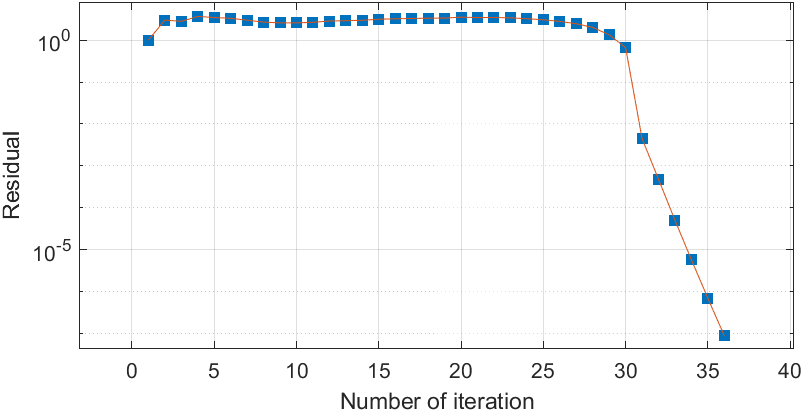
\includegraphics[width=1\textwidth]{residual.png} % first figure itself      
    \end{minipage}\hfill
    \begin{minipage}{0.5\textwidth}
        \centering
        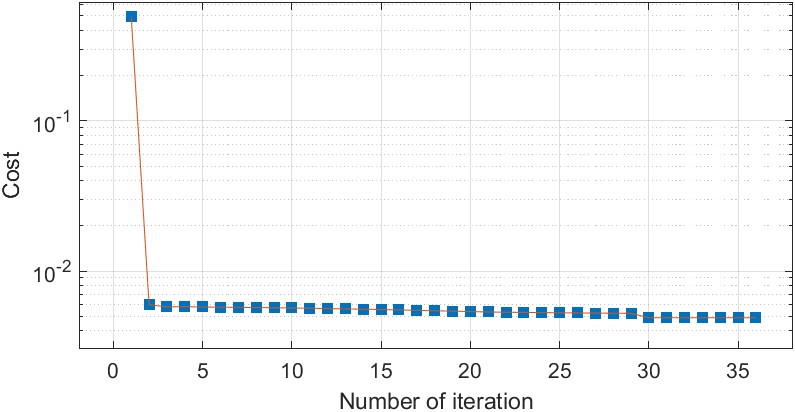
\includegraphics[width=1\textwidth]{cost.png} % second figure itself        
    \end{minipage}
    \caption{Residual and Cost of the problem vs number of iterations of the algorithm}
\end{figure}

   We can appreciate that, despite the convergence of the algorithm, the residual behavior tends to have low variations until the thirtieth iteration, where the residual descends significantly. On the other hand, the cost of the problem tends to stabilize before the fifth iteration. Table 1. presents a summarize of the numerical evolution of our algorithm through the 35 iterations. We point out that until the iteration number $25$, the residual tends to decrease slowly. However, the number of null elements of the optimal control $u$ tends to increase until a stabilization. As null elements of u we refer to the entries $u(\cdot,\cdot)$ which are small enough to be considerate as zero.

\begin{table}[h]
    \centering
    \begin{tabular}{|c|c|c|c|c|}
    \hline
    It. &Null elements in $u$ &Residual     & Cost\\ 
    \hline
1  & 0    & 3.0087     & 0.005972\\  
2  & 1696 & 2.7933     & 0.005772  \\
3  & 776  & 3.6731     & 0.0057934 \\
4  & 2520 & 3.4509     & 0.0057655 \\
5  & 2708 & 3.3105     & 0.0057486 \\
10 & 3244 & 2.658      & 0.0056555 \\
15 & 3808 & 3.2191     & 0.00551   \\
20 & 4452 & 3.4425     & 0.0053416 \\
25 & 4804 & 2.7981     & 0.0052616 \\
30 & 4876 & 0.0044843  & 0.0048893 \\
31 & 4876 & 0.00047814 & 0.0048893 \\
32 & 4876 & 5.0666e-05 & 0.0048893 \\
33 & 4876 & 5.735e-06  & 0.0048893 \\
34 & 4876 & 6.9444e-07 & 0.0048893 \\
35 & 4876 & 8.8643e-08 & 0.0048893 \\
    \hline
\end{tabular}
\caption{Numerical results of the experiment incorporated.}
\end{table}
\subsection{Varying problem parameters} In this section we present the results of varying individually the parameters $\alpha, \beta$ and $q$ present in \eqref{P}. In the first case, we vary only $\alpha$, taking $\beta=2e-3$, $p=2$, $\lambda=1e-4$ and $\gamma=2500$. Table 2 summarizes our results:
\begin{table}[h]
    \centering
    \begin{tabular}{|c|c|c|c|c|}
    \hline
    $\alpha$ & Optimal cost & Null elements in $u$ & Number of iterations\\
    \hline
    0.0175&0.0055555&4796&49\\
    0.0125&0.0053958&6076&43\\
    0.01  & 0.0052986 &6676  & 43  \\
    0.005 &0.0050413 &7900  &44\\
    0.003 &0.0048888 &8460  &45\\
    0.00125 & 0.0046883 & 9056 & 47\\
    \hline
    \end{tabular}
    \caption{Variations of $\alpha$}
\end{table}

Notice that, as $\alpha$ decrease, the null elements in $u$ tends to increase and the number of iterations are relatively constant. Next, we vary $\beta$, taking $\alpha=0.0175$, $p=2$, $\lambda=1e-4$ and $\gamma=2500$. Results are summarized in the Table 3.
\begin{table}[h]
    \centering
    \begin{tabular}{|c|c|c|c|c|}
    \hline
    $\beta$ & Optimal cost & Null elements in $u$ & Number of iterations\\
    \hline
    0.00125&0.0053617&4192&44\\
    0.0007&0.0052083&3684&40\\
    0.00025  & 0.0050747 &3028  & 37  \\
    0.000075&0.0050198&2556&35\\
    5e-5&0.0050099&1788&35\\
    1e-5 &0.0049953 &496  &60\\
    1e-6 &0.0049921 &88  &37\\    
    \hline
    \end{tabular}
    \caption{Variations of $\beta$}
\end{table}

The effect that we report over the sparsity of $u$ in this case is the opposite of the previous case: here, as $\beta$ tends to decrease, the null elements in $u$ tends to decrease too. Finally, we vary the parameter $p$, taking $\alpha=0.01, \beta=3e-4, \lambda=1e-4$ and $\gamma=2500$. The results are summarized in Table 4.
\begin{table}[h]
    \centering
    \begin{tabular}{|c|c|c|c|c|}
    \hline
    $p$ & Optimal cost & Null elements in $u$ & Number of iterations\\
    \hline
    1.1&00.0048639&1196&42\\
    1.4&0.0048828&3012&37\\
    2&0.0049158&5144&37\\
    3.5  & 0.0049367 &5392  & 37  \\
    5&0.0049464&5336&38\\
    5.2&0.0049477&5296&38\\   
    \hline
    \end{tabular}
    \caption{Variations of $p$}
\end{table}

We notice that, as $p$ tends to increase, the sparcity of $u$ tends to increase too. The number of iterations again are relatively constant, and in general, the optimal cost in each reported cases tends to present small variations during the variation of the parameters. The graphical solutions of each group of experiments, as its graphical supports are presented in Figures 3, 4 and 5.\\

\subsection{Varying regularization parameters}
In this sub section we report our numerical experiments at which the regularization parameters are tested, keeping fixed the parameters of the problem. The main idea of this section is to observe the behavior of the optimal control as $\gamma$ tends to infinity and $\lambda$ tends to zero. First of all, we present the numerical results of varying $\gamma$, keeping $\alpha=0.01, \beta=0.0003, p=2$ and $\lambda=1e-4$.  Results are summarized in Table 5.  
\begin{table}[h].
    \centering
    \begin{tabular}{|c|c|c|c|c|}
    \hline
    $\gamma$ & Optimal cost & Null elements in $u$ & Number of iterations\\
    \hline
    1500&0.0049158&5144&37\\
    3500&0.0049158&5144&37\\
    6000&0.0049158&5144&37\\
    10000  & 0.0049158 &5144  & 37  \\
    1e5&0.0049158&5144&37\\ 
    \hline
    \end{tabular}
    \caption{Varations of $\gamma$}
\end{table}

\begin{figure}[H]
    \centering
    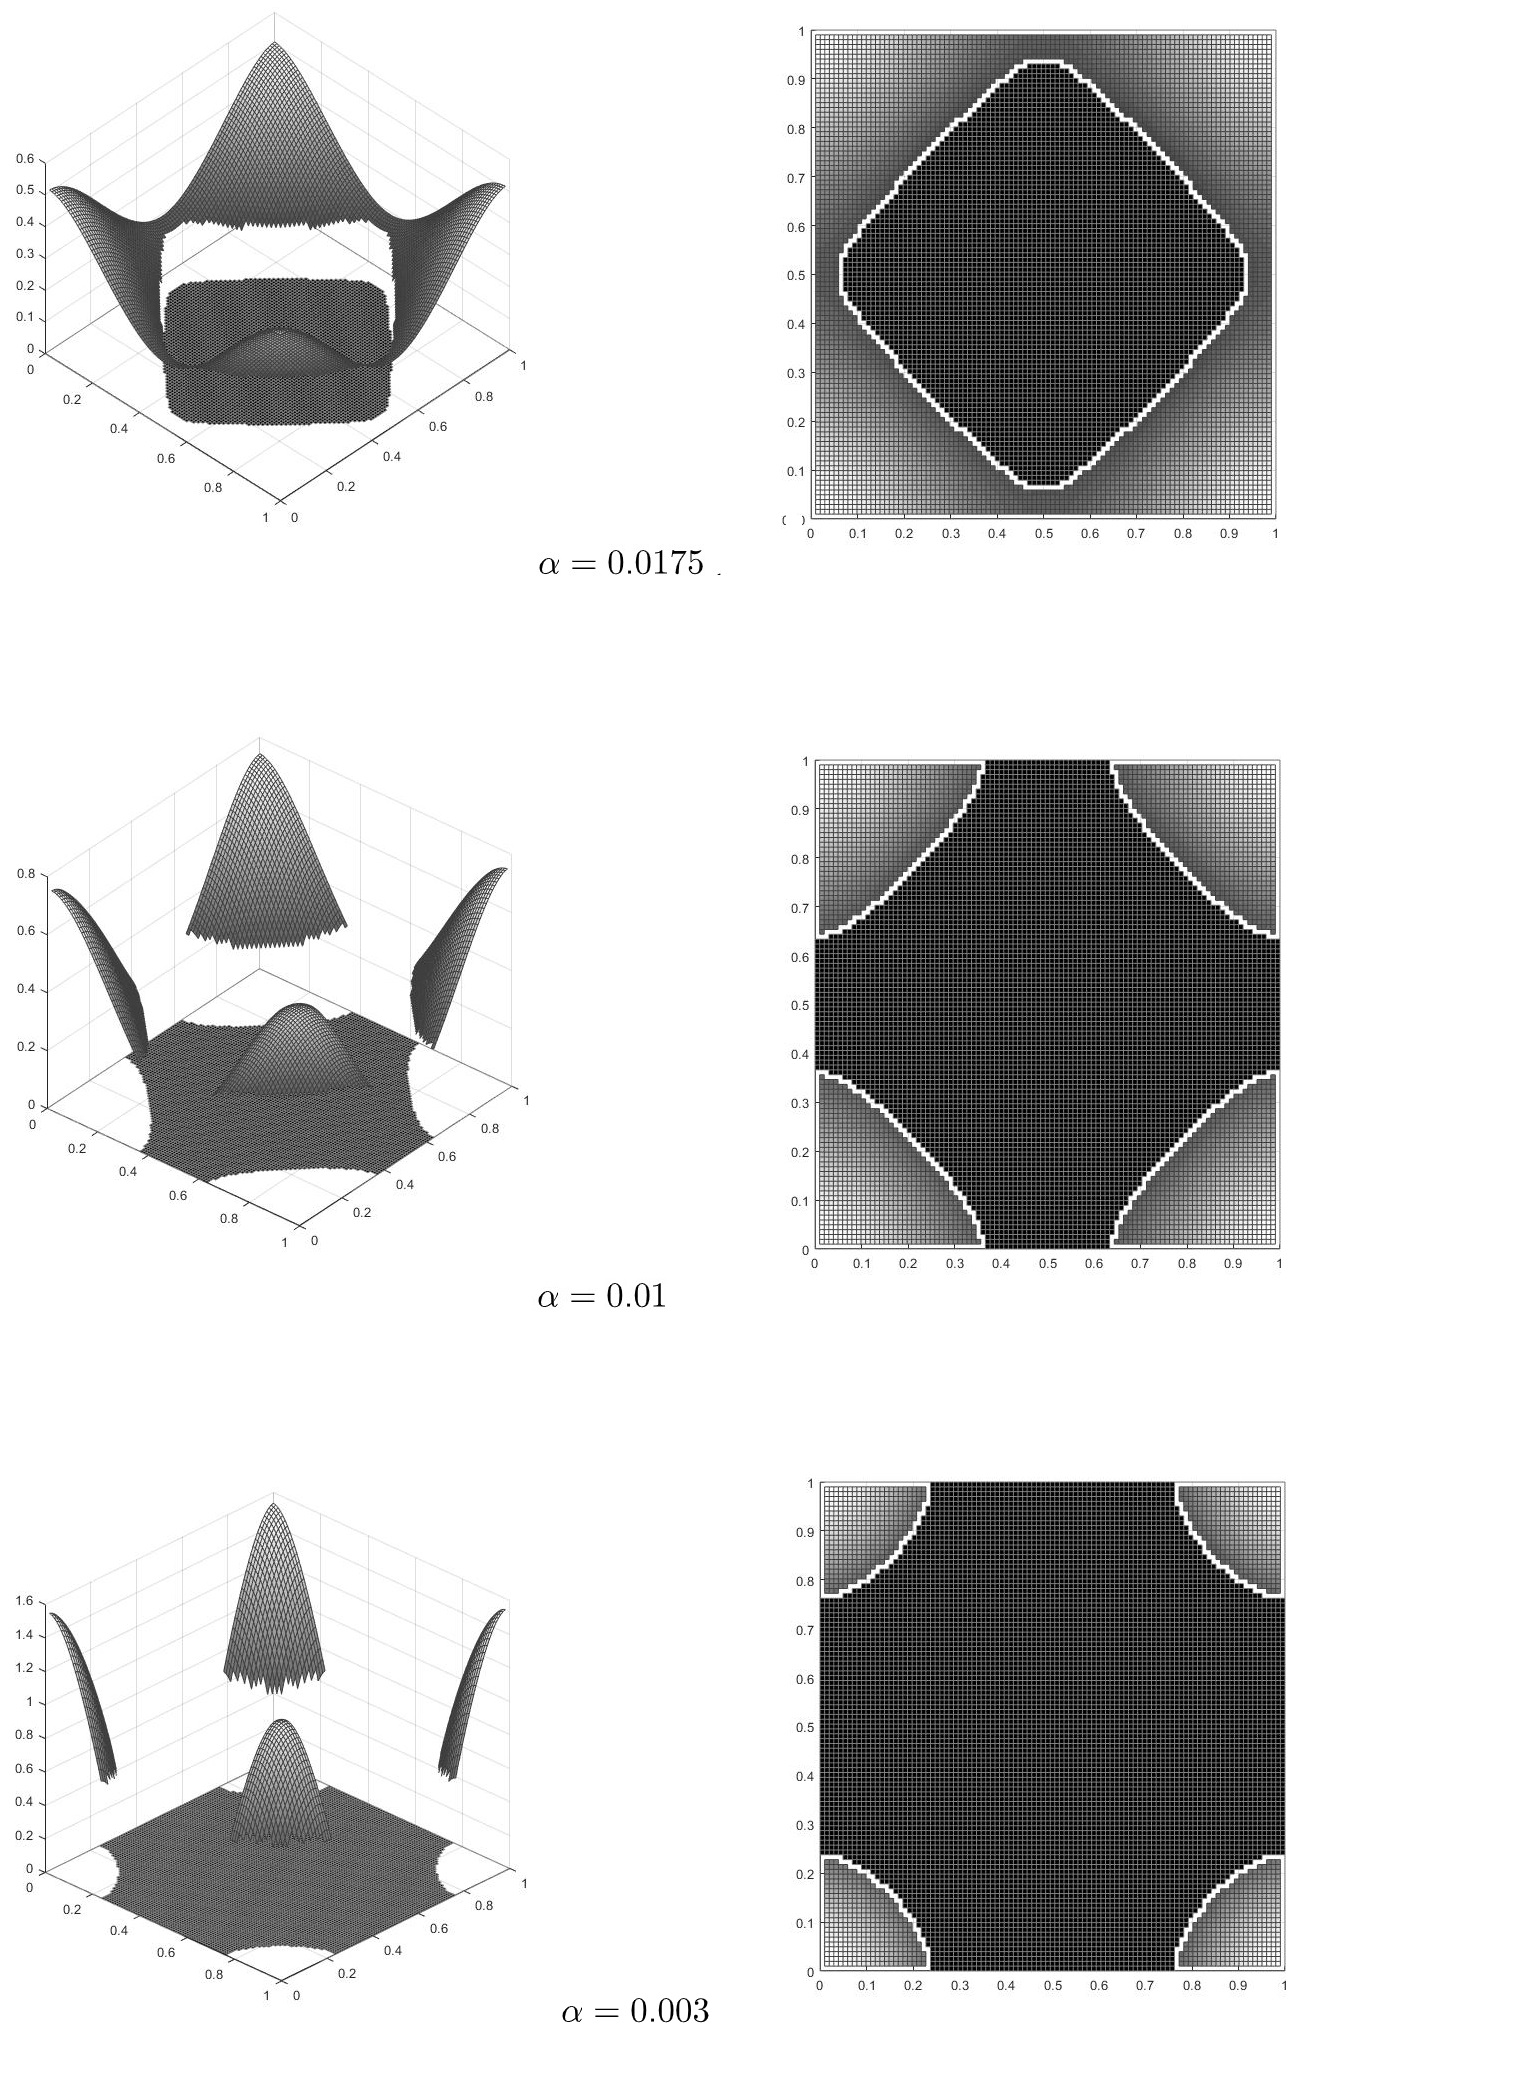
\includegraphics[scale=0.35]{matrizaa.jpg}
    \caption{Graphics of the optimal control $u$ (first column) and their supports (second column) as $\alpha$ varies. The first row correspond to the solution when $\alpha=0.0175$, the second corresponds to $\alpha=0.01$ and third corresponds to $\alpha=0.003$. We notice that, as $\alpha$ decrease, the support of function decrease, too.}
\end{figure}




\begin{figure}[H]
    \centering
    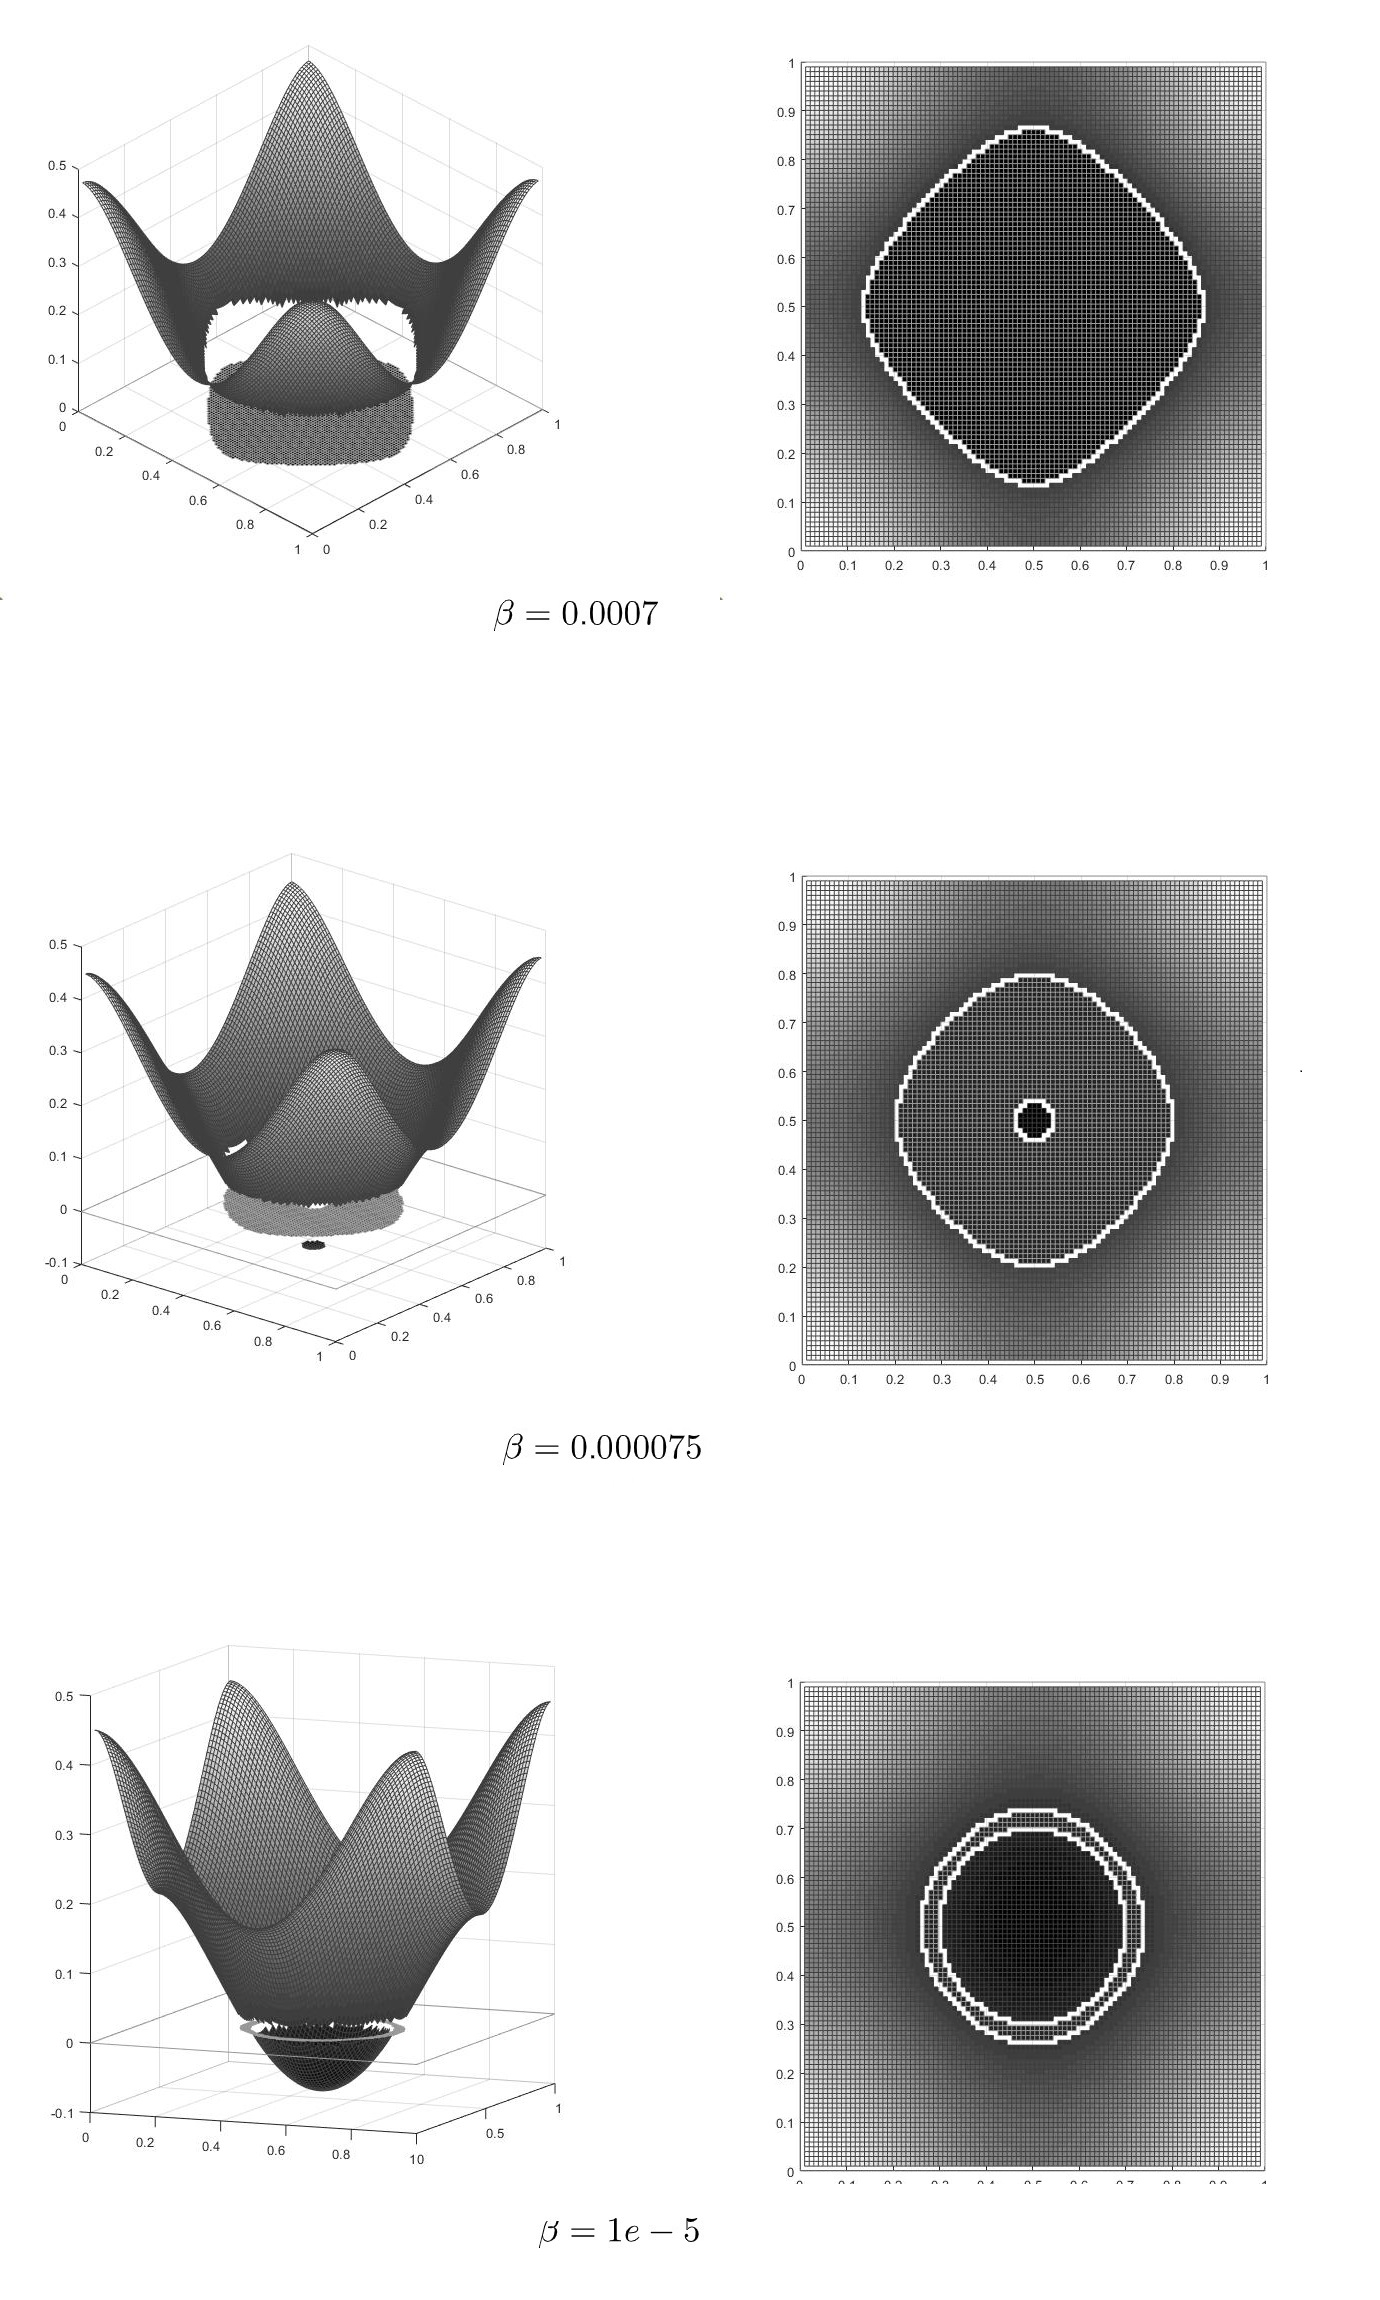
\includegraphics[scale=0.35]{matrizb.jpg}
    \caption{Graphics of the optimal control $u$ (first column) and their supports (second column) as $\beta$ varies. The first row correspond to the solution when $\beta=0.0007$, the second corresponds to $\beta=0.000075$ and third corresponds to $\beta=1e-5$. We notice that, as $\beta$ decrease, the support of function increase.}    
\end{figure}


\begin{figure}[H]
    \centering
    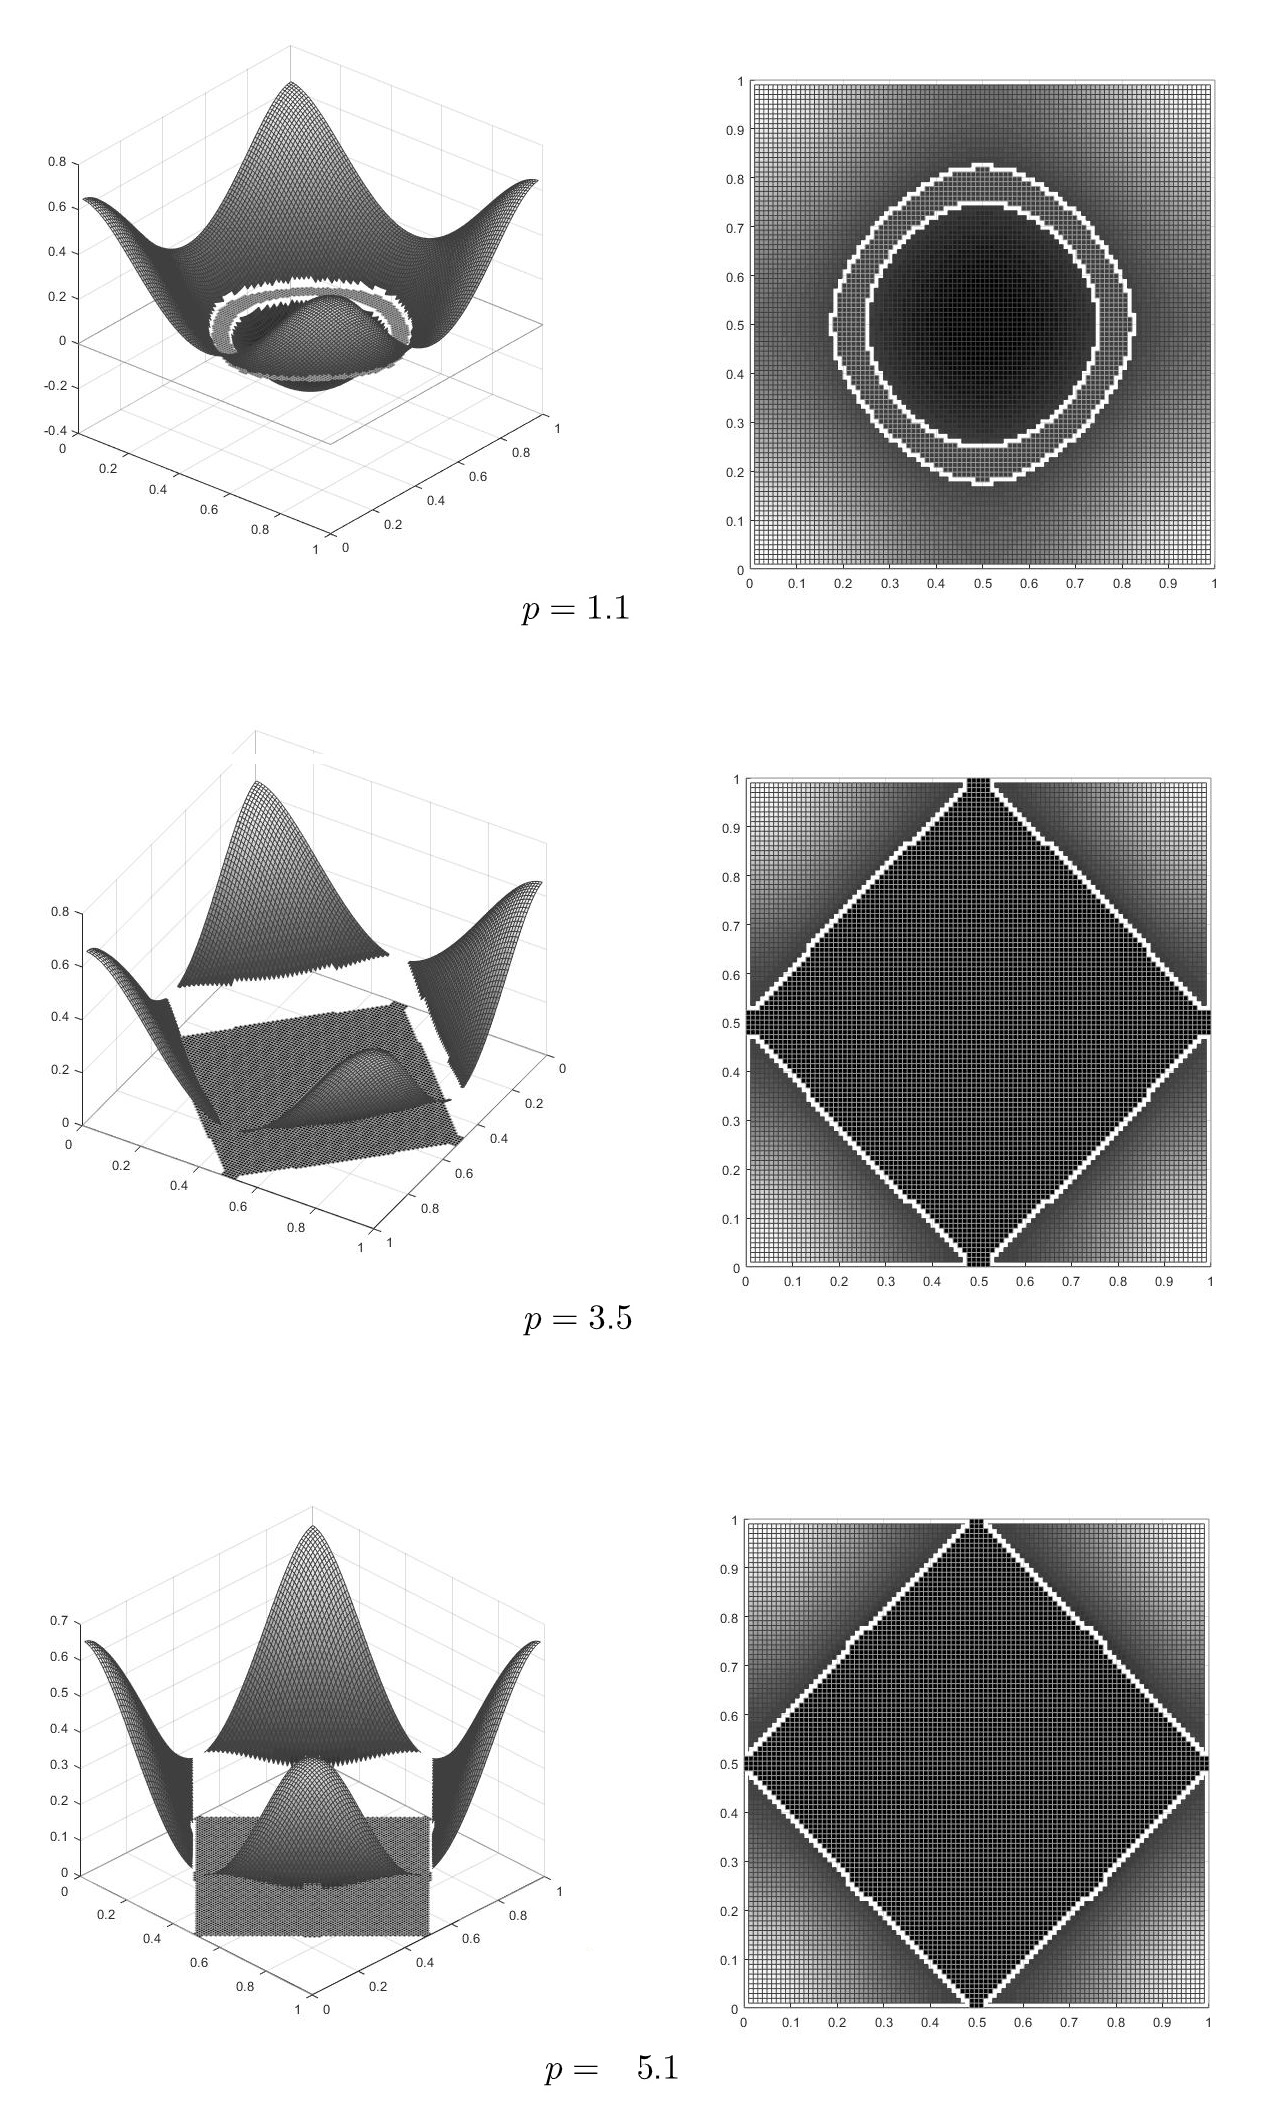
\includegraphics[scale=0.35]{matrizp.jpg}
    \caption{Graphics of the optimal control $u$ (first column) and their supports (second column) as $p$ varies. The first row correspond to the solution when $p=1.1$, the second corresponds to $p=3.5$ and third corresponds to $p=5.1$. We notice that, as $p$ increase, $q=\frac{1}{p}$ decrease and the support of function decrease, too.}   
\end{figure}

\newpage

We can see that the  optimal cost of the problem, such as  the null elements of $u$ tends to be constant. Even the number of iterations tends to be constant, too. The graphic of the optimal control and state for the higher value of $\gamma$ are presented in Figure 6.
\begin{figure}[h]
    \centering
    \begin{minipage}{0.5\textwidth}
        \centering
        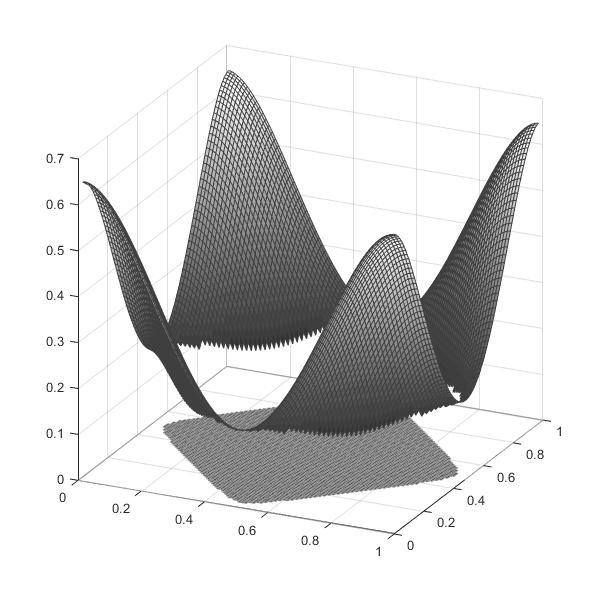
\includegraphics[width=0.7\textwidth]{ug.jpg} % first figure itself      
    \end{minipage}\hfill
    \begin{minipage}{0.5\textwidth}
        \centering
        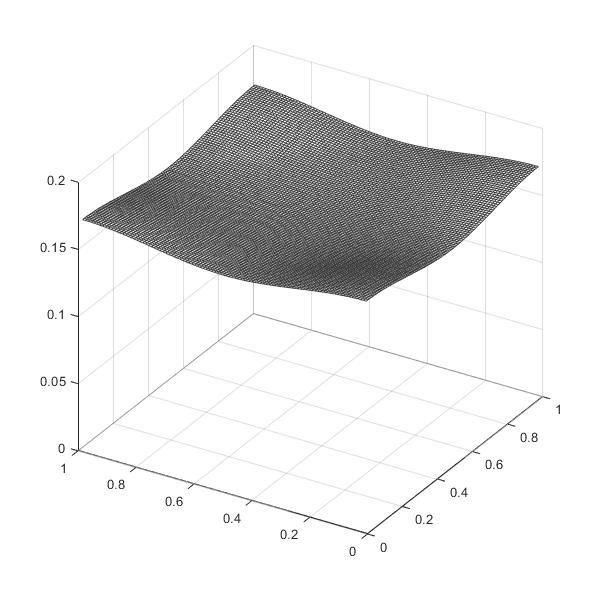
\includegraphics[width=0.7\textwidth]{yg.jpg} % second figure itself        
    \end{minipage}
    \caption{Optimal control (left) and state (right) for the limit problem when $\gamma=1e5$.}
\end{figure}



For the test of $\lambda$, we take $c_1=1000$ and $c_2=50$, $\alpha=1e-3, \beta=2e-5, p=2$. Numerical results are presented in Table 6.

\begin{table}[h]
    \centering
    \begin{tabular}{|c|c|c|c|c|}
    \hline
    $\lambda$ & Optimal cost & Null elements in $u$ & Number of iterations\\
    \hline
    1e-4&0.0049671&5544&38\\
    1e-5&0.004967&5528&62\\
    1e-6&0.004967&5528&62\\
    1e-7& 0.004967 &5528  & 62\\  
    \hline
    \end{tabular}
    \caption{Variations of $\lambda$}
\end{table}
 Again, we can see that as $\lambda$ tends to decrease, optimal cost and null elements in $u$ tends to be constant. Graphical solutions are shown in Figure 7 
\begin{figure}[h!]
    \centering
    \begin{minipage}{0.5\textwidth}
        \centering
        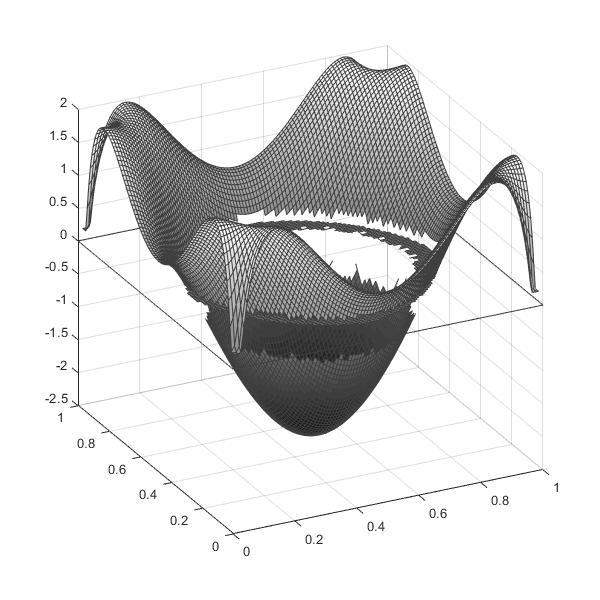
\includegraphics[width=0.7\textwidth]{ul.jpg} % first figure itself      
    \end{minipage}\hfill
    \begin{minipage}{0.5\textwidth}
        \centering
        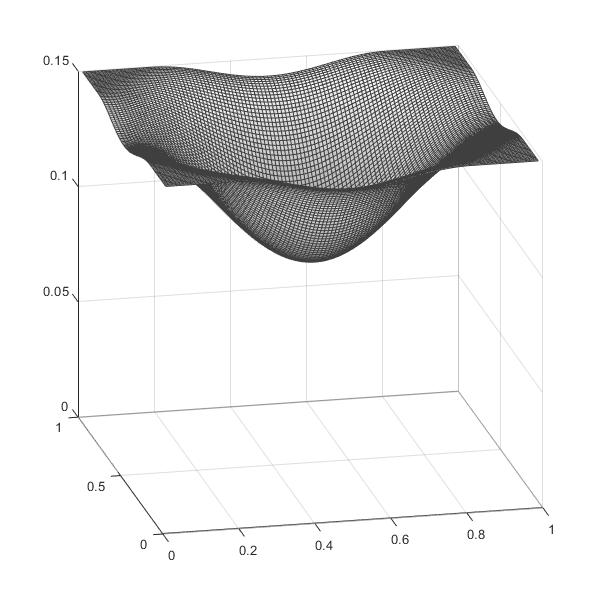
\includegraphics[width=0.7\textwidth]{yl.jpg} % second figure itself        
    \end{minipage}
    \caption{Optimal control (left) and state (right) for the limit problem when $\lambda=1e-7$.}
\end{figure}


\newpage
\newpage


The experiments presented before always report that $y$ is point wise strictly inside the bounds $y_a=-1$ and $y_b=0.2$, and therefore we can not see the real utility of Lavrentiev regularization in our problem; this motivate us to change the upper bound to $y_b=0.15$ and test again  our algorithm, varying $\lambda$ and reporting the number of point wise evaluations of $y$ which are significantly equal to $0.15$. Here, we take  $c_1=1000$ and $c_2=50$, $\alpha=1e-3, \beta=2e-5, p=2$. Table 7 report the variation of the active restrictions that are reached by $y$, as $\lambda$ tends to decrease
\begin{table}[h]
    \centering
    \begin{tabular}{|c|c|c|c|c|}
    \hline
    $\lambda$ & Optimal cost & Active restrictions in $y$ & Number of iterations\\
    \hline
    1e-3&0.0043199&0&28\\
    1e-4&0.0043155&848&43\\
    1e-5&0.0043182&896&62\\
    1e-6&0.0043187&906 &91\\  
    1e-7&0.0043185&904&67\\
    1e-8&0.0043185&904&67\\
    \hline
    \end{tabular}
\end{table}
We observe that as $\lambda$ tends to zero, the number of active restrictions of $y$ tends to increase until a stabilization of $904$. The optimal cost, however, tends to be constant. This show us that the state at the limit of $\lambda$ satisfies all the point wise  restrictions, even which equality. Now, the multiplier $\mu$ introduced in the optimal system associated to the semi smooth scheme developed in this section should satisfies the complementary conditions. Figures 8 and 9 show the optimal state and multiplier $\mu$ in the limit case $\lambda=1e-7$.
\begin{figure}[h]
    \centering
    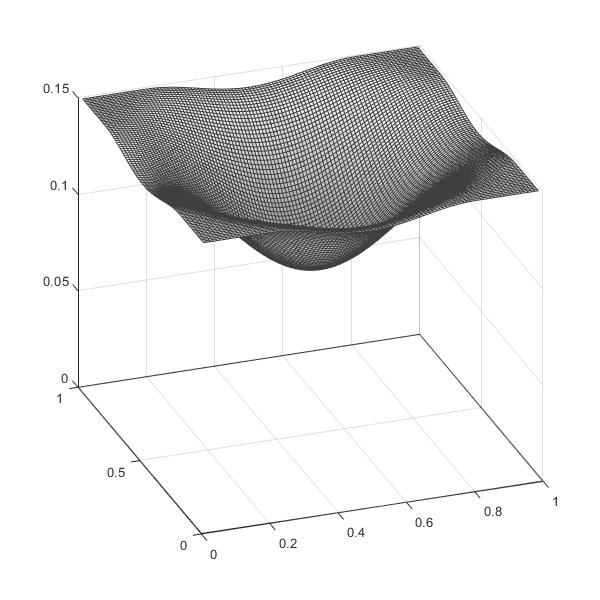
\includegraphics[scale=0.3]{yact.jpg}
    \caption{Optimal state in the limit case $\lambda=1e-7$}
\end{figure}

\newpage

\begin{figure}[H]
    \centering
    \begin{minipage}{0.5\textwidth}
        \centering
        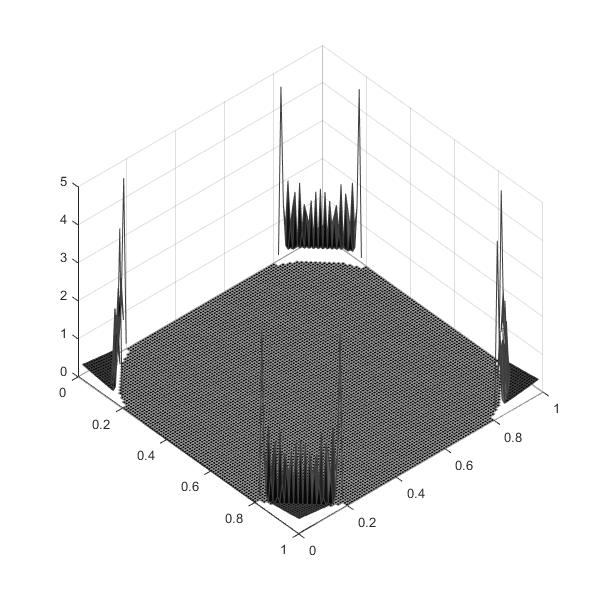
\includegraphics[width=0.8\textwidth]{mu.jpg} % first figure itself      
    \end{minipage}\hfill
    \begin{minipage}{0.5\textwidth}
        \centering
        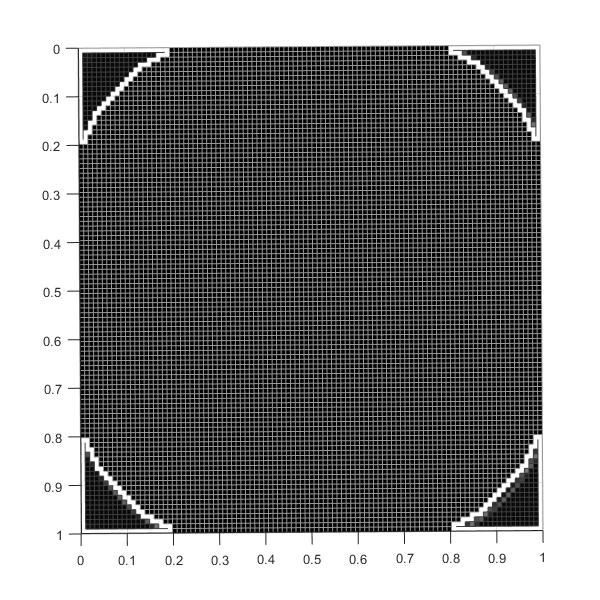
\includegraphics[width=0.8\textwidth]{musop.jpg} % second figure itself        
    \end{minipage}
    \caption{Graphic of the multiplier $\mu$ and its support}
\end{figure}

We can see that the support of $\mu$ coincides with the zones of $y$ which are strictly inside the interval $[-1,0.15]$. This implies that the complementary condition is satisfied in this region. On the other hand, when $y$ is active, $\mu$ takes other values than $zero$.

\section{Conclusions}
In this work we can prove the existence of solution for problem \eqref{P} using a Convex regularization of the problem, also called $\Gamma$ regularization. The point wise restrictions impossed to the state are carry out using a Lavrentiev regularization, which allow us to generate a family of convexified problems $(PC_{\lambda_n})_{n\in \mathbb{N}}$ which their solutions tend to a optimal solution for \eqref{P}.  For the numerical treatment of the problem, we developed a Semi-smooth Newton method with Lagrange multipliers in $L^2(\om)$, which ease the numerical treatment of the problem. This multipliers appear from the Lavrentiev regularization of \eqref{P}. The semi-smooth scheme has been developed from an optimal system arisen from the DC theory, using a Huber type regularization for the treatment of the nonconvexity of the problem.\\

Experimentally, we confirm that the quasinorm term present in \eqref{P} induces over $u$ sparsity in regions of the domain of the control that does not have necessary zero measure. This can be corroborated in the experiments when $\alpha$ and $\beta$ are varied separately. Is a interesting fact that the exponent of the quiasinorm $q=1/p$ influence over the sparsity of $u$ too.\\

Respect to the regularization parameters $\gamma$ and $\lambda$, we see that, through their variations tending to a limit ($\gamma\to \infty$ and $\lambda\to 0$) the numerical results tend to stabilize in an optimal solution; fact that we expected to have. In the case of the point wise restrictions of $y$, we see that $\mu$ satisfies the complementary conditions imposed in the optimal systems.\\

The globalization of the semi-smooth Newton method should be used for improving the numerical development of the algorithm. This fact is not used in the present investigation and might be considered in future researchs.






\begin{thebibliography}{99}

\bibitem{ambrosetti}
Ambrosetti, A.; Prodi, G., A Primer of Nonlinear Analysis. Cambridge, Cambridge University Press 1993. VIII, 171 pp., £ 25.00 H/b. ISBN 0-521-37390-5 (Cambridge Studies in Advanced Mathematics 34)

\bibitem{combettes}
Bauschke, H. H., and Combettes, P. L. Convex Analysis and Monotone Operator Theory in Hilbert Spaces, 2011. CMS books in mathematics).

\bibitem{bik}
Maïıtine Bergounioux, Kazufumi Ito and Karl Kunisch. “Primal-dual Strategy for Constrained Optimal Control Problems”. In: SIAM Journal on Control and Opti- mization 37, no 4 (1999), pp. 1176-1194.

\bibitem{bk}
Maïıtine Bergounioux and Karl Kunisch. “On the structure of Lagrange multipliers for state-constrained optimal control problems”. En: Systems Control Lett. 48 (mar. de
2003), pp. 169-176.

\bibitem{casas}
Eduardo Casas. Control of an Elliptic Problem with Pointwise State Constraints. In: SIAM Journal on Control and Optimization 24. (1986), pp. 1309-1318.

\bibitem{casasclason}
Eduardo Casas, Christian Clason, and Karl Kunisch. Parabolic control problems in measure spaces
with sparse solutions. SIAM Journal on Control and Optimization, 51(1):28-63, 2013.

\bibitem{casas-delosreyes}
Casas, Eduardo, Juan Carlos De Los Reyes, and Fredi Tröltzsch. "Sufficient second-order optimality conditions for semilinear control problems with pointwise state constraints." SIAM Journal on Optimization 19.2 (2008): 616-643.

\bibitem{casas-kunisch}
Casas, Eduardo, and Karl Kunisch. "Optimal control of semilinear parabolic equations with non-smooth pointwise-integral control constraints in time-space." Applied Mathematics \& Optimization 85.1 (2022): 12.

\bibitem{casaskruse}
Casas, Eduardo, Florian Kruse, and Karl Kunisch. "Optimal control of semilinear parabolic equations by BV-functions." SIAM Journal on Control and Optimization 55.3 (2017): 1752-1788.



\bibitem{delosreyes}
J.C De los Reyes. Theory of PDE-constrained optimization. Springer, Berlin, (2015).

\bibitem{dihn}
Pham Dinh, Tao and Le Thi and  Hoai An, Recent Advances in DC Programming and DCA,Springer Berlin Heidelberg, (2014), pp. 1-37.

\bibitem{donoho}
D.L.Donoho. ,Compressed sensing. IEEE Trans.Inform.Theory,52, 2006, pp. 1289-1306

\bibitem{eck}
I. Ekeland and R. Temam, Convex Analysis and Variational Problems, SIAM, Philadelphia, 1999.

\bibitem{hintkun}
M. Hintermüller and Karl Kunisch, Stationary optimal control problems with pointwise state constraints, SIAM Journal on Optimization, (2007). 

\bibitem{hinttv}
M. Hintermüller and T. Wu, Nonconvex TVq-Models in Image Restoration: Analysis and
a Trust-Region Regularization Based Superlinearly Convergent Solver, preprint, 2012.

\bibitem{ito-kunish}
K. Ito y K. Kunisch. Optimal control with $L^p(\om)$, $p \in [0,1)$, control cost. SIAM, J. Control optim. 2014 Society for Industrial y Applied Mathematics Vol.52,No.2,
2014, pp. 1251-1275.

\bibitem{kr}
Karl Kunisch and Arnd Rösch. “Primal-dual active set strategy for a general class
of constrained optimal control problems”. En: SIAM Journal on Optimization 13.2
(2002), pp. 321-334.

\bibitem{merino}
Pedro Merino. A difference-of-convex functions approach for sparse PDE optimal control problems with nonconvex costs. Comput Optim Appl 74. Springer Science+Business Media. (2019), pags. 225-258.

\bibitem{merino1}
Pedro Merino. A Semismooth Newton Method for Regularized Lq-quasinorm Sparse Optimal Control Problems. Numerical Mathematics and Advanced Applications ENUMATH 2019. Springer Nature Switzerland. (2019), pags. 723-731.

\bibitem{meyer1}
Chr. Meyer, U. Prüfert and F. Tröltzsch. “On two numerical methods for state-
constrained elliptic control problems”. In: Optimization Methods and Software 22.6
(2007), pp. 871-899.

\bibitem{mifflin}
R. Mifflin, Semismooth and semiconvex functions in constrained optimization, SIAM J. Control Optim., 15, (1977), pp. 959–972.

\bibitem{qi}
L. Qi, C-differential operators, C-differentiability and generalized Newton methods, Research Report
AMR96/5, School of Mathematics, University of New South Wales, Sydney, New South Wales, Australia (1996).


\bibitem{qisun}
L. Qi and J. Sun, A nonsmooth version of Newton’s method,
jMath. Programming, 58, (1993), pp 353-367

\bibitem{rock} 
Tyrrell R. Rockafellar, R., Convex analysis, Princeton Mathematical Series, (1970).

\bibitem{stadler}
Georg Stadler, Elliptic optimal control problems with L1-control cost and applications for the placement of control devices, Computational Optimization and Applications, Volume 44, (2009), pp. 159-181

\bibitem{trol}
  F. Tröltzsch and J. Sprekels. Optimal Control of Partial Differential Equations: Theory, Methods, and Applications,Graduate studies in mathematics,American Mathematical Society, (2010)


\bibitem{ulbrich}
Ulbrich, Michael. Semismooth Newton methods for variational inequalities and constrained optimization problems in function spaces. Society for Industrial and Applied Mathematics, 2011.

\bibitem{valkonen}
Christian Clason and Tuomo Valkonen, Introduction to Nonsmooth Analysis and Optimization. 	arXiv:2001.00216, 2023

\bibitem{vogel}
 Curtis Vogel, Computational Methods for Inverse Problems, Society for Industrial and Applied Mathematics, (2002)

\bibitem{vossen}
 Georg Vossen, and Maurer, H., On $L^1$‐minimization in optimal control and applications to robotics,Optimal Control Applications and Methods, Volume 27, (2006), pp. 301-321. 
\end{thebibliography}
\end{document}






